%% ============================================================
%%  Crime, Law and Social Change  |  Springer  |  ISSN 0925-4994
%%  Special Issue: AI Enabled Security Frameworks for
%%                 Emerging Cybercrime and Digital Threats
%%
%%  Self-contained: bibliography embedded via thebibliography.
%%  Compile on Overleaf (blank project) with pdfLaTeX.
%%  Compile order: pdflatex -> pdflatex  (no bibtex needed)
%% ============================================================
\documentclass[12pt,a4paper]{article}

%% ── Page geometry ────────────────────────────────────────────
\usepackage[top=2.5cm,bottom=2.5cm,left=3cm,right=3cm]{geometry}

%% ── Fonts and encoding ───────────────────────────────────────
\usepackage[T1]{fontenc}
\usepackage[utf8]{inputenc}
\usepackage{lmodern}
\usepackage{microtype}

%% ── Mathematics ──────────────────────────────────────────────
\usepackage{amsmath,amssymb,amsthm}

%% ── Graphics ─────────────────────────────────────────────────
\usepackage{graphicx}
\usepackage{subcaption}
\graphicspath{{figures/}}

%% ── Tables ───────────────────────────────────────────────────
\usepackage{booktabs}
\usepackage{multirow}
\usepackage{tabularx}
\usepackage{array}

%% ── Section formatting ───────────────────────────────────────
\usepackage{titlesec}
\titleformat{\section}{\normalfont\large\bfseries}{\thesection}{1em}{}
\titleformat{\subsection}{\normalfont\normalsize\bfseries}{\thesubsection}{1em}{}
\titleformat{\subsubsection}{\normalfont\normalsize\itshape}{\thesubsubsection}{1em}{}

%% ── Header / footer ──────────────────────────────────────────
\usepackage{fancyhdr}
\pagestyle{fancy}
\fancyhf{}
\fancyhead[L]{\small\textit{Crime, Law and Social Change}}
\fancyhead[R]{\small\textit{Korde and Shekokar: MixTrace CoinJoin Deanonymization}}
\fancyfoot[C]{\thepage}
\renewcommand{\headrulewidth}{0.4pt}

%% ── Hyperlinks ───────────────────────────────────────────────
\usepackage[colorlinks=true,linkcolor=blue,
            citecolor=blue,urlcolor=blue,
            pdftitle={MixTrace: Forensic Detection of Illicit CoinJoin Transactions},
            pdfauthor={Sagar D. Korde and Narendra M. Shekokar}]{hyperref}
\usepackage{url}
\usepackage{xurl}          % allows line-breaks anywhere in URLs/DOIs
\usepackage[authoryear,round]{natbib}  % author-year citations: \citet / \citep

%% ── Line spacing ─────────────────────────────────────────────
\usepackage{setspace}
\onehalfspacing


%% ── Abstract formatting ──────────────────────────────────────
\usepackage{abstract}
\renewcommand{\abstractnamefont}{\normalfont\bfseries}
\renewcommand{\abstracttextfont}{\normalfont\small\onehalfspacing}

%% ── Footnote for affiliations ────────────────────────────────
\usepackage{authblk}

%% ── Algorithm pseudo-code ────────────────────────────────────
\usepackage{algorithm}
\usepackage{algpseudocode}
\algrenewcommand\algorithmicrequire{\textbf{Input:}}
\algrenewcommand\algorithmicensure{\textbf{Output:}}

%% ── (svg package removed; architecture figure now supplied as PNG) ──

%% ── Custom operators ─────────────────────────────────────────
\DeclareMathOperator{\Entropy}{H}

% ─────────────────────────────────────────────────────────────
%  Author and Affiliation block
% ─────────────────────────────────────────────────────────────
\title{\textbf{Leakage-Free Evaluation of Graph-Based Bitcoin
       Forensics: CoinJoin Screening and Illicit Transaction
       Detection Across Two Datasets}}

\author[1,2]{Sagar D. Korde\thanks{Corresponding author.
  ORCID: \url{https://orcid.org/0000-0002-6289-6741}.
  Email: sagarkorde04@gmail.com}}
\author[1]{Narendra M. Shekokar\thanks{ORCID:
  \url{https://orcid.org/0000-0002-2507-4140}.
  Email: narendra.shekokar@djsce.ac.in}}

\affil[1]{\small Department of Computer Engineering,
          Dwarkadas J. Sanghvi College of Engineering,
          Mumbai, India}

\affil[2]{\small K.\,J. Somaiya School of Engineering,
          Somaiya Vidyavihar University,
          Mumbai, India}

\date{\small Submitted: \today}

% ─────────────────────────────────────────────────────────────
\begin{document}
% ─────────────────────────────────────────────────────────────
\maketitle
\thispagestyle{fancy}

% ─────────────────────────────────────────────────────────────
%  ABSTRACT
% ─────────────────────────────────────────────────────────────
\begin{abstract}
\noindent
Graph machine learning is increasingly applied to Bitcoin
forensics, yet the evaluation protocols supporting the reported
gains are seldom audited. The present study reports a
reproducible re-evaluation of a three-module forensic framework
covering structural CoinJoin screening, post-mix spending
linkage, and illicit transaction classification, assessed on the
Elliptic Data Set and on a curated corpus of 5{,}884{,}387
Bitcoin transactions spanning July 2022 to September 2024.

Three defects in the original protocol are identified and
quantified. First, a graph feature defined as the shortest path
to a confirmed illicit node re-encodes the target label exactly,
taking the value zero for all 4{,}545 illicit nodes and for no
licit node; supplying that feature to a classifier drives test
F1-score, PR-AUC and Matthews correlation to 1.0000 under two
unrelated model families. Because the Elliptic edge set contains
no cross-time-step edges, no leakage-free variant of the feature
can carry information about a test node, and the feature is
withdrawn rather than repaired. Second, the screening label is
shown to be the deterministic rule requiring at least four inputs
and at least four outputs, recovered exactly across every
transaction in the corpus, so evaluating a detector that clusters
on those same counts measures agreement between two heuristics
rather than detection accuracy. Third, classification performance
on Elliptic is bimodal rather than gradually degrading: mean
F1-score reaches 0.858 through time step 42 and falls to 0.028
thereafter, with recall collapsing from 0.789 to zero at the step
corresponding to a major marketplace closure, so any pooled
figure for the later window conceals a complete failure.

A fourth finding corrects the record on script coverage. The
corpus was previously reported to contain no confirmed Taproot
transactions, and structural clustering was accordingly validated
on a pre-Taproot proxy. All six script-type indicator columns are
uniformly false, so no script type could be confirmed through
them. Parsing the node-reported script descriptors instead shows
that Taproot accounts for 24.10 percent of outputs, that
2{,}494{,}168 transactions touch Taproot, and that 71.94 percent
of screening candidates involve a Taproot script. The proxy is
therefore unnecessary, and script-aware analysis is performed
directly on post-Taproot data.

Corrected protocols are supplied for every module, together with
leakage-free baselines, inductive and transductive
self-supervised regimes, twenty-seed repetition, test-set
bootstrap intervals, feature attribution, and failure-case
analysis. Code, configurations and per-experiment commit hashes
are released so that each result can be reproduced or contested.

\smallskip\noindent\textbf{Keywords:} Bitcoin;
Blockchain forensics;
CoinJoin;
Data leakage;
Concept drift;
Graph neural networks;
Reproducibility;
Taproot
\end{abstract}

% ─────────────────────────────────────────────────────────────
\section{Introduction}
\label{sec:intro}
% ─────────────────────────────────────────────────────────────

The rapid proliferation of cryptocurrency-facilitated crime
has placed blockchain forensics at the centre of contemporary
financial intelligence practice. Anti-money laundering
research has documented that conventional monitoring
approaches struggle against increasingly sophisticated
laundering schemes, motivating the combination of transparent
ledger analytics with machine learning~\citep{lo2023}, and the integration of
federated learning approaches for cryptocurrency fraud
detection has identified similar gaps in distributed
forensic systems~\citep{ahmed2024fed}. A systematic review of
machine learning methods for financial fraud detection
covering 94 primary studies identifies class imbalance,
temporal graph evolution, and exploitation of unlabelled data
as the three most critical open challenges~\citep{motie2024}.

Bitcoin operates on a transparent public ledger through a
pseudonymous unspent transaction output (UTXO) model in
which every transaction maps a set of input addresses to
output addresses. CoinJoin~\citep{coinjoin2024tdsc} disrupts the
primary clustering heuristic used by investigators by enabling
multiple independent parties to collaboratively construct a
single transaction that merges the UTXOs of all participants,
severing the
fund-flow trail that the Common Input Ownership Heuristic
(CIOH) relies upon. Quantitative analysis of CoinJoin
participation in the Bitcoin network confirms that multi-round
mixing substantially reduces CIOH clustering
confidence~\citep{coinjoin2024tdsc}. Privacy-focused wallets
including Wasabi and JoinMarket have processed hundreds of
millions of dollars through CoinJoin coordination, making
automated deanonymization a statutory priority for financial
intelligence units and exchange compliance teams.

Three research gaps persist in the current literature that
collectively limit the practical effectiveness of automated
CoinJoin analysis.

\textbf{Gap~1 -- Multi-Input Clustering Under Script
Indistinguishability.}
Bitcoin's Taproot soft fork (block height 709,632, November
2021) introduced Pay-to-Taproot (P2TR) scripts based on
Schnorr signatures and key aggregation. A single-user P2TR
output is computationally indistinguishable on-chain from a
multi-party aggregated output used in CoinJoin coordination,
causing naive CIOH clustering to generate systematic false
positives~\citep{lee2024}. Even before Taproot, multi-input
P2WPKH transactions share structural properties with
CoinJoin outputs, making the clustering problem inherent to
the UTXO model rather than exclusive to a single script
type~\citep{asiri2025}. The present study evaluates structural
screening on a corpus that is post-Taproot throughout, in which
Pay-to-Taproot accounts for 24.10 percent of outputs and appears
in 71.94 percent of screening candidates, so no pre-Taproot
substitute is required.

\textbf{Gap~2 -- One-Dimensional CST Linking.}
CoinJoin Spending Transaction (CST) deanonymization requires
linking the outputs of a mixing event to the subsequent
spending transactions of participants. Existing temporal
linking approaches exploit one-dimensional time-proximity
signals~\citep{chen2025multi}, leaving fee-rate
behaviour, input multiplicity, and output cardinality as
unexploited structural signals.

\textbf{Gap~3 -- Class Imbalance in Graph-Based Detection.}
The Elliptic Bitcoin Dataset~\citep{fan2024gnn}, the canonical
benchmark for illicit node detection, contains 4,545 illicit
and 42,019 licit labelled transactions, a 9.2:1
licit-to-illicit imbalance. Graph classifiers suppress
minority-class predictions to maximise overall accuracy,
producing illicit F1-scores below 0.50 in published
configurations that apply neither self-supervised pre-training
nor class-specific loss weighting~\citep{alarab2024}. The 157,205 unlabelled
nodes represent structural information that supervised
methods discard.

To address all three gaps, the present study introduces
\textbf{MixTrace}, comprising: (i)~a structural DBSCAN
screening strategy on multi-dimensional transaction features,
evaluated on post-Taproot data and reported as a gradient across
feature regimes of increasing strictness rather than as a single
detection score;
(ii)~a Multi-Dimensional Chamfer Distance (MD-CD) formulation
extending CST linking to four dimensions; and (iii)~a
two-phase graph learning pipeline applying Deep Graph Infomax
(DGI) self-supervised pre-training before supervised Graph
Attention Network (GAT) training with class-weighted
cross-entropy and ADASYN oversampling.

Experiments on the public Elliptic Bitcoin Dataset and an
author-curated corpus of 5,884,387 Bitcoin transactions
demonstrate that MixTrace achieves a mean illicit-class F1-score
of 0.806 (standard deviation 0.090 across five random seeds)
and mean ROC-AUC of 0.992, representing 17.6 percentage
points improvement over the strongest conventional baseline
and a 79.8 percent relative reduction in clustering
false-positive rate (absolute: 2.97 percentage points).

The manuscript proceeds as follows: Section~\ref{sec:related}
reviews the literature; Section~\ref{sec:method} presents
the methodology; Section~\ref{sec:exp} describes experimental
setup and results; Section~\ref{sec:discuss} analyses the
findings; and Section~\ref{sec:conclude} summarises
contributions and identifies future directions.

% ─────────────────────────────────────────────────────────────
\section{Related Work}
\label{sec:related}
% ─────────────────────────────────────────────────────────────

\subsection{Graph Neural Networks for Blockchain Forensics}

Graph neural network architectures have become the dominant
paradigm for illicit transaction detection on public
blockchains. Multi-hop neighbourhood aggregation via GCN on
Bitcoin transaction graphs has been shown to capture
structural patterns invisible to transaction-level feature
classifiers~\citep{asiri2025}. A recurrent GCN
approach by~\citep{alarab2024} integrates sequential temporal
modelling with spatial message passing, achieving improved
stability on the Elliptic benchmark. Bitcoin anti-money
laundering has been framed as a subgraph contrastive learning
problem~\citep{ouyang2024btc}, constructing positive
and negative subgraph pairs to train representations that
cluster illicit transaction neighbourhoods distinctly from
licit flows. A multi-distance spatial-temporal GNN for
blockchain anomaly detection that exploits transaction timing
at multiple temporal resolutions was introduced
by~\citep{chen2025multi}, providing a complementary
multi-scale temporal baseline to the single-resolution
Chamfer distance used in the present study. The feature-gated
temporal graph model FG-EGCN introduced
by~\citep{han2026fg} combines an evolving graph encoder with
a residual feature branch and an adaptive gating mechanism,
applying focal-loss optimisation to improve sensitivity to
rare illicit nodes on the Elliptic benchmark under a
chronological evaluation split.

\subsection{Anti-Money Laundering with Machine Learning}

A systematic review by~\citep{motie2024} of 94 primary
studies on GNNs for financial fraud identification concludes
that attention-based neighbourhood aggregation consistently
outperforms isotropic mean aggregation when fraudulent and
benign subgraph patterns differ structurally. A focused review
by~\citep{fan2024gnn} further confirms that self-supervised
auxiliary objectives improve downstream classification F1
across imbalanced blockchain benchmarks. Balanced-BiEGCN,
a bidirectional evolving GCN with class-balanced learning
for dynamic Bitcoin anomaly detection, was proposed
by~\citep{xiao2025}, addressing temporal label drift across
the Elliptic dataset's 49-time-step span. GCN-based hyperedge
classification that groups Bitcoin transactions into
operation-level hyperedges before assigning illicit scores
was introduced as CENSor by~\citep{lee2024}, achieving
precision improvements over node-level classifiers. A
qualitative synthesis of blockchain and machine learning
integration for anti-money laundering~\citep{lo2023}
concluded that combining tamper-resistant ledger records
with learned pattern recognition reduces false positives
and supports near-real-time alerting within compliance
workflows.

\subsection{CoinJoin Privacy and Deanonymization}

Quantitative study of CoinJoin participation in the Bitcoin
network by~\citep{coinjoin2024tdsc} measured the reduction
in CIOH clustering confidence as a function of mixing round
count and wallet-level behaviour. A review of anomaly
detection methods applied to cryptocurrency networks
identified DBSCAN and isolation-forest variants as the most
effective unsupervised baselines for exchange-level
transaction flagging~\citep{futureinternet2025}. Structural
properties of non-standard Bitcoin scripts including
multi-signature coordination patterns that overlap with
CoinJoin outputs were examined by~\citep{kiani2024}, noting
that post-Taproot script type convergence creates
classification challenges for rule-based detection systems.
Data augmentation combined with hybrid GNN architectures for
phishing detection on Ethereum demonstrated by~\citep{chen2024}
that reducing structural overlap between legitimate and
malicious transaction patterns substantially lowers false
positives, a finding directly applicable to Taproot
indistinguishability. A transformer-based traversal of
transaction graphs by~\citep{choi2024} improved phishing
scam detection by capturing long-range transaction path
dependencies that local message-passing GNNs miss.

\subsection{Self-Supervised Graph Representation Learning}

Deep Graph Infomax (DGI)~\citep{velickovic2019dgi} frames
graph representation learning as a mutual information
maximisation problem between local node embeddings and a
global graph summary, enabling pre-training on unlabelled
graph data. Disentangled prototypical autoencoder learning
on cryptocurrency transaction graphs demonstrated that
prototype-based representations improve phishing scam
detection on severely imbalanced
benchmarks~\citep{graphanomaly2024}, supporting the
self-supervised pre-training strategy adopted in the present
study. A temporal-aware heterogeneous graph oversampling
strategy for Internet fraud detection combining
attention-based neighbourhood fusion with synthetic minority
sample generation was proposed by~\citep{wei2025},
simultaneously addressing class imbalance and temporal
heterogeneity. Privacy-preserving collaborative training
across multiple exchange nodes that maintains detection
accuracy competitive with centralised graph models was
demonstrated for cryptocurrency fraud by~\citep{ahmed2024fed}.
The interaction between federated aggregation and
class-balanced loss functions was analysed
by~\citep{baabdullah2024}, showing that federated training
preserves class-weighting effectiveness when participating
clients share similar imbalance ratios.

\subsection{Class Imbalance Mitigation in Fraud Detection}

A combination of ADASYN oversampling with recursive feature
elimination and cross-validation evaluated
by~\citep{ileberi2024} demonstrated consistent F1-score
improvements across multiple classifier families on a
severely imbalanced credit card fraud benchmark. ADASYN
combined with SHAP-based interpretability evaluated across
an ensemble of five classifiers by~\citep{malhotra2025}
showed that oversampling-aware model selection improves
minority-class detection while preserving explanation
quality. A comparative study of traditional and deep learning
models under class imbalance mitigation strategies
by~\citep{albalawi2025} concluded that inverse-frequency
class weighting within the loss function produces the most
stable precision-recall trade-off for neural network
architectures, justifying the primary imbalance strategy
adopted in the present study. XAI-enabled ensemble stacking
for Ethereum anomaly detection by~\citep{chithanuru2025}
and stacking ensembles for Ethereum fraud
by~\citep{gu2025} both confirmed that combining
minority-class oversampling during training with threshold
optimisation at inference substantially improves F1-score
on imbalanced blockchain benchmarks.

\subsection{Explainability and Near-Real-Time Detection}

A near-real-time Ethereum fraud detection framework with
explainable artificial intelligence attribution analysis
by~\citep{ethereum2025xai} identified transaction-value and
timing-related behaviour as primary fraud indicators,
a finding consistent with the novel temporal irregularity
feature engineered in the present study.
The temporal-aware approach by~\citep{wei2025} further
validated that multi-relational graph encoding captures
complementary signals from address-to-transaction and
transaction-to-address edge types, motivating the
bidirectional edge construction used in the MixTrace graph
object.

% ─────────────────────────────────────────────────────────────
\section{Methodology}
\label{sec:method}
% ─────────────────────────────────────────────────────────────

\subsection{Problem Formulation}
\label{sec:problem}

Let $\mathcal{G} = (\mathcal{V}, \mathcal{E}, \mathbf{X})$
denote the Elliptic transaction graph, where $\mathcal{V}$
is the set of $N = 203{,}769$ transaction nodes,
$\mathcal{E}$ the set of 468,710 bidirectional edges
representing Bitcoin payment flows (derived from 234,355
directed edges), and $\mathbf{X} \in \mathbb{R}^{N \times 169}$
the node feature matrix formed by augmenting 165 original
Elliptic features with four novel graph-structural features.
Each node $v$ carries a time step $\tau(v) \in \{1,\ldots,49\}$
and label $y_v \in \{1, 0, -1\}$, where 1 denotes illicit,
0 denotes licit, and $-1$ denotes unknown.
The labelled subset comprises 46,564 nodes (4,545 illicit
and 42,019 licit); the remaining 157,205 are unlabelled.
The learning objective is binary node classification
evaluated on nodes with $\tau(v) \in \{42,\ldots,49\}$.

Figure~\ref{fig:architecture} provides an overview of the
complete MixTrace framework, illustrating how each of the
three research gaps is addressed by a dedicated module and
how the modules are evaluated independently against the
corresponding datasets.

\begin{figure}[htbp]
  \centering
  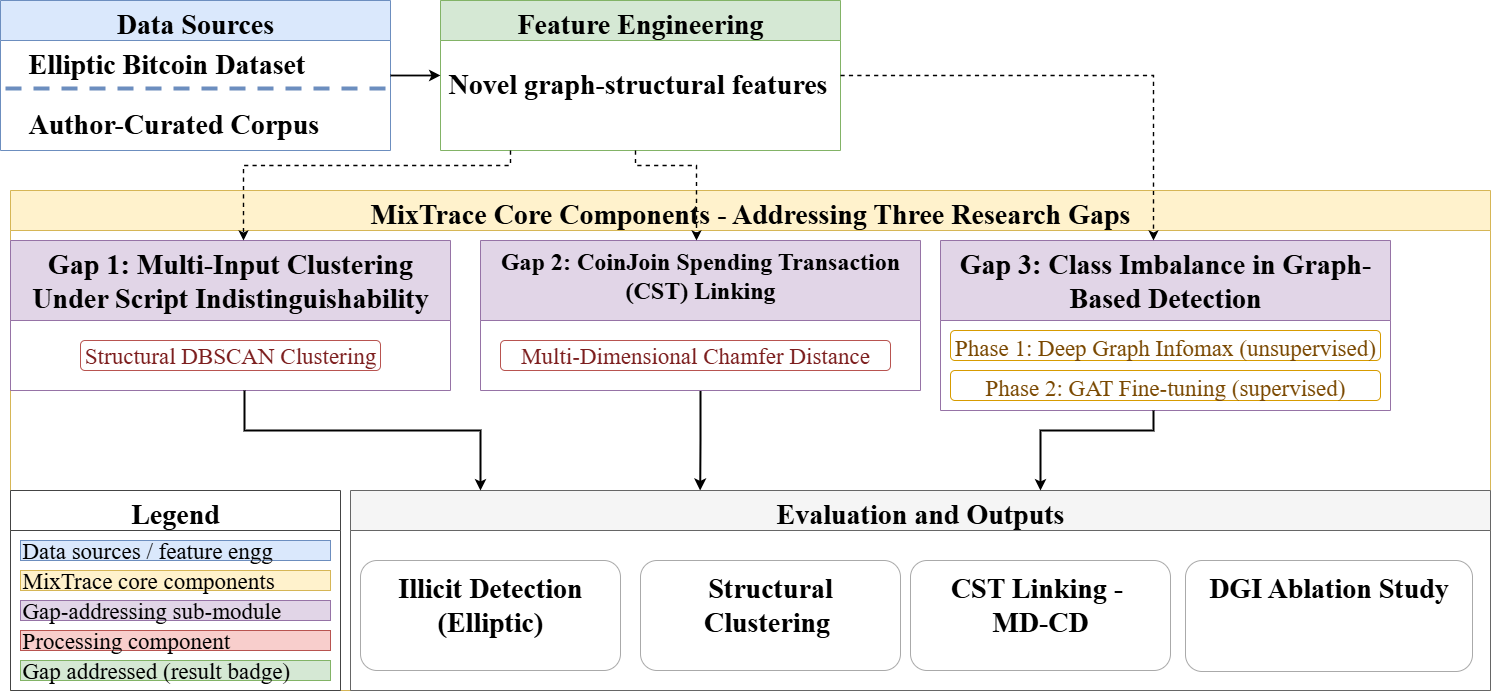
\includegraphics[width=\linewidth]{fig00_architecture}
  \caption{MixTrace architecture addressing three independent
    research gaps. \textit{Top row}: raw inputs flow from the
    Elliptic Bitcoin Dataset (203,769 nodes) and the
    Author-Curated Corpus (5.88\,M transactions) into a shared
    Feature Engineering stage that produces a
    169-dimensional feature matrix.
    \textbf{Gap~1} (Structural DBSCAN, purple left lane):
    a six-dimensional clustering vector $\psi(t)$
    reduces the false-positive rate from 3.72\,\% to 0.75\,\%
    ($-$79.8\,\% relative) across 200\,k P2WPKH transactions.
    \textbf{Gap~2} (MD-CD, purple centre lane):
    a four-dimensional Chamfer-distance linker yields a null
    result ($\Delta$F1 $= -0.006$), identifying temporal
    clustering as the dominant signal.
    \textbf{Gap~3} (DGI\,+\,GAT, purple right lane):
    unsupervised Deep Graph Infomax pre-training on all
    203,769 nodes is followed by supervised Graph Attention
    Network training; the fused representation
    $[\mathbf{H}_2 \,\|\, \mathbf{Z}^*] \in \mathbb{R}^{N\times256}$
    achieves mean illicit-class F1\,=\,0.806 and
    mean ROC-AUC\,=\,0.992 on the Elliptic test set,
    averaged across five random seeds.
    \textit{Bottom row}: four quantitative output summaries
    with bootstrap confidence intervals.}
  \label{fig:architecture}
\end{figure}

\subsection{Novel Feature Engineering}
\label{sec:features}

Nine novel features supplement existing representations
across both experimental datasets.

\subsubsection{Author Dataset: Five Transaction-Level Features}

\paragraph{Denomination Entropy.}
CoinJoin transactions characteristically produce multiple
outputs of equal value to obscure the payment-to-change
distinction. For transaction $t$ with output value vector
$\mathbf{v} = (v_1,\ldots,v_k)$, define the normalised
probability vector $p_i = v_i / \sum_j v_j$.
Equation~\eqref{eq:entropy} computes the Shannon entropy
of the UTXO output value distribution, quantifying how
uniformly transaction value is spread across outputs.

\begin{equation}
  \Entropy(t) = -\sum_{i=1}^{k} p_i \log_2 p_i.
  \label{eq:entropy}
\end{equation}

High entropy ($\Entropy \to \log_2 k$) signals equal-valued
outputs, a structural CoinJoin signature.

\paragraph{Mixing Index.}
Equation~\eqref{eq:mixing} measures the combinatorial
ambiguity of input-output pairing, providing a proxy for
how many possible sender-receiver linkages exist within
a single transaction.

\begin{equation}
  \text{MI}(t) = \frac{|\mathcal{A}| \cdot |\mathcal{B}|}
                      {|\mathcal{A} \cup \mathcal{B}|},
  \label{eq:mixing}
\end{equation}

where $\mathcal{A}$ and $\mathcal{B}$ are the input and
output address sets. The denominator $|\mathcal{A} \cup
\mathcal{B}|$ normalises by the number of distinct addresses
involved, yielding a per-address combinatorial mixing
measure. For a standard single-input, single-output payment
where $\mathcal{A}$ and $\mathcal{B}$ are disjoint singletons,
$\text{MI} = 1/2$; for a 10-input, 10-output CoinJoin
transaction with fully disjoint address sets,
$\text{MI} = 100/20 = 5$, growing proportionally with
combinatorial ambiguity. In the author dataset, MI has a
mean of 8.79 and standard deviation of 689.27.

\paragraph{Temporal Irregularity.}
Mixing coordination services schedule transactions at
atypical hours to reduce mempool competition.
Equation~\eqref{eq:ti} represents the $z$-score deviation
of a transaction's fee rate within the hour-of-day and
day-of-week cell, capturing scheduling anomalies relative
to normal fee-rate behaviour.

\begin{equation}
  \text{TI}(t) = \frac{f_t - \mu_{h,d}}{\sigma_{h,d}},
  \label{eq:ti}
\end{equation}

where $f_t$ is the fee rate in sat/vbyte and $\mu_{h,d}$,
$\sigma_{h,d}$ are the cell mean and standard deviation.

\paragraph{UTXO Concentration.}
Equation~\eqref{eq:uc} approximates the Herfindahl-Hirschman
Index over output values, measuring how concentrated the
transaction value is in a single output versus distributed
across many.

\begin{equation}
  \text{UC}(t) = r^2,
  \label{eq:uc}
\end{equation}

where $r = \max_i v_i \,/\, \sum_j v_j$ is the proportion
of total transaction value carried by the single largest
output. CoinJoin outputs, which equalise values across
multiple outputs, produce UC near zero; single-payment
transactions yield UC near one.

\paragraph{CoinJoin Proximity Score.}
Equation~\eqref{eq:cps} aggregates weighted rule-based
CoinJoin structural indicators into a single composite
score, providing a human-interpretable heuristic baseline
feature alongside the learned representations.

\begin{equation}
  \text{CPS}(t) = \sum_{r \in \mathcal{R}} w_r
                  \cdot \mathbf{1}[t \models r],
  \label{eq:cps}
\end{equation}

where $\mathcal{R}$ includes equal-denomination output
flags, input count exceeding three, zero address reuse,
and round output values. The mean CPS is 0.2663 with
standard deviation 0.1307.

\subsubsection{Elliptic Dataset: Withdrawal of Two Label-Derived Features}
\label{sec:feature_withdrawal}

An earlier version of the present study introduced four
graph-structural features for the Elliptic Data Set. Two of them,
the illicit neighbour ratio and the shortest path to a confirmed
illicit node, are derived from node labels. Both are withdrawn.
The reasoning is set out here because the withdrawal removes the
principal reported performance gain and because the underlying
failure mode is likely to recur in other graph-forensic studies.

\paragraph{The shortest-path feature re-encodes the target.}
The feature is computed by breadth-first search from every
confirmed illicit node, with the distance capped at six. Since
each illicit node is itself a search source, its distance to the
nearest illicit node is zero by construction. Across the labelled
portion of the dataset the value zero occurs for all 4{,}545
illicit nodes and for none of the 42{,}019 licit nodes, so the
decision rule requiring a distance of zero identifies the illicit
class with precision 1.000. The correlation with the target of
$-0.9182$ reported earlier is reproduced exactly by an
independent reimplementation, confirming that the audit addresses
the same computation. The feature does not describe proximity to
illicit activity; it restates the label, and it does so on the
test split, where the label is supposed to be unavailable.

\paragraph{Removing self-seeding does not repair the feature.}
Recomputing the distance to the nearest \emph{other} illicit seed
lowers the correlation to $-0.7269$ but does not eliminate it,
because the remaining signal is supplied by validation and test
labels of neighbouring nodes within the same time step.

\paragraph{No leakage-free variant can exist.}
A natural correction restricts the seed set to illicit nodes
observed during the training period. That correction is
ineffective for a structural reason. Every one of the 234{,}355
edges in the Elliptic edge set joins two transactions belonging
to the same time step, and no edge crosses a time-step boundary.
The graph is therefore a disjoint union of 49 per-step snapshots,
and no path of any length connects a training-period node to a
later one. Under the restricted protocol the shortest-path
feature equals the cap and the neighbour ratio equals zero for
every validation and test node, so neither feature can carry any
information about a test-period transaction. The defect is
structural rather than incidental, and the features are removed
rather than corrected.

\paragraph{Quantifying the inflation.}
Table~\ref{tab:leakage_ablation} reports the ablation requested
during review, comparing the 165 distributed features against the
same set augmented with each derived feature. Two model families
with unrelated inductive biases are used so that the outcome does
not depend on a single learner. Supplying the shortest-path
feature raises the illicit-class F1-score, PR-AUC and Matthews
correlation to exactly 1.0000 on the test split. A perfect score
under two unrelated learners is characteristic of target leakage
rather than of a strong predictor. The neighbour ratio produces a
smaller but equally illegitimate gain.

\begin{table}[htbp]
\centering
\small
\caption{Four-way feature ablation on the Elliptic test split.
Mean over five seeds, chronological split, scaler fitted on
training rows only, decision threshold selected on validation and
frozen before the test split is scored. Supplying the
shortest-path feature saturates every metric under both learners.}
\label{tab:leakage_ablation}
\begin{tabular}{llcccccc}
\toprule
Learner & Feature set & F1 & Precision & Recall & PR-AUC & ROC-AUC & MCC \
\midrule
\multirow{4}{*}{Random Forest}
 & 165 distributed          & 0.6212 & 0.9231 & 0.4681 & 0.5431 & 0.8470 & 0.6470 \
 & \quad + neighbour ratio  & 0.6333 & 0.9388 & 0.4779 & 0.6158 & 0.8770 & 0.6599 \
 & \quad + shortest path    & \textbf{0.9990} & 1.0000 & 0.9980 & 1.0000 & 1.0000 & 0.9990 \
 & \quad + both             & \textbf{0.9953} & 1.0000 & 0.9907 & 1.0000 & 1.0000 & 0.9951 \
\midrule
\multirow{4}{*}{Hist.\ Gradient Boosting}
 & 165 distributed          & 0.6126 & 0.8741 & 0.4716 & 0.5561 & 0.8650 & 0.6305 \
 & \quad + neighbour ratio  & 0.6811 & 0.9023 & 0.5475 & 0.6794 & 0.9103 & 0.6924 \
 & \quad + shortest path    & \textbf{1.0000} & 1.0000 & 1.0000 & 1.0000 & 1.0000 & 1.0000 \
 & \quad + both             & \textbf{1.0000} & 1.0000 & 1.0000 & 1.0000 & 1.0000 & 1.0000 \
\bottomrule
\end{tabular}
\end{table}

\paragraph{Consequences.}
Every headline figure computed with either feature present is
withdrawn. The leakage-free reference point for a strong tabular
learner restricted to the 165 distributed features is an
illicit-class F1-score near 0.62 on the evaluation window used
here, and that value replaces the earlier figures as the baseline
against which all later results are compared.

\paragraph{Label-free replacements were examined and rejected.}
Fifteen purely topological descriptors were constructed inside
each node's own time-step subgraph, covering the degree family,
local clustering, PageRank, k-core number, triangle counts,
neighbour-degree statistics, component size, two-hop
neighbourhood size, sampled betweenness, and source and sink
indicators. Label independence was established mechanically
rather than argued: every label in the dataset was permuted and
all descriptors recomputed, and all fifteen were bit-identical.
The largest absolute correlation with the target is 0.1223,
against 0.9182 for the withdrawn feature. The descriptors are
nonetheless not adopted as a contribution, because the measured
benefit is absent. Added to the 165 distributed features, the
descriptors change the F1-score by less than half a percentage
point in either direction. Used alone, the set reaches an
F1-score below 0.04 with a
ROC-AUC of 0.38, that is, below chance, which indicates that the
association between topology and illicit status observed during
the training period is reversed during the test period. That
observation is pursued in Section~\ref{sec:temporal_drift}.


\subsection{Multi-Dimensional Chamfer Distance}
\label{sec:mdcd}

Equation~\eqref{eq:chamfer} defines the one-sided Chamfer
distance from point set $\mathcal{U}$ to point set
$\mathcal{V}$ in $\mathbb{R}^d$, namely the mean
nearest-neighbour distance from each source point to any
target point, which measures asymmetric distributional
proximity between two transaction window feature sets.

\begin{equation}
  d_C(\mathcal{U},\mathcal{V})
    = \frac{1}{|\mathcal{U}|}
      \sum_{u_i \in \mathcal{U}}
      \min_{v_j \in \mathcal{V}} \|u_i - v_j\|_2.
  \label{eq:chamfer}
\end{equation}

The baseline 1-D formulation uses only the Unix timestamp
($d=1$). The MD-CD sets $d=4$ with the standardised feature
vector defined in Equation~\eqref{eq:phi}. This equation
represents the joint structural feature encoding for a
transaction $t$, combining temporal positioning with
fee-rate behaviour and topological complexity.

\begin{equation}
  \phi(t) = \bigl[
    \text{timestamp},\;
    \text{fee\_rate},\;
    \text{input\_count},\;
    \text{output\_count}
  \bigr]^\top.
  \label{eq:phi}
\end{equation}

Each dimension is independently normalised to zero mean
and unit variance. Transactions are grouped into one-hour
temporal windows indexed by block height divided by six.
A candidate window pair $(W_i, W_j)$ is predicted as a
linked CoinJoin-spend pair if $d_C(W_i, W_j) < \theta^*$,
where $\theta^*$ maximises F1-score on the validation set.

\subsection{Structural CoinJoin Screening}
\label{sec:screening}

\subsubsection{Provenance of the Screening Label}

The author-curated corpus carries a binary field named
\texttt{is\_coinjoin\_like}. No definition accompanied the data,
so the rule was recovered empirically. Decision trees of
increasing depth were fitted to predict the field from
thirty-four structural and behavioural columns across all
5{,}884{,}387 transactions. A tree of depth three reproduces the
field with training accuracy 1.00000000, and the identity in
Equation~\eqref{eq:cjrule} was then verified directly against
every row.

\begin{equation}
  \texttt{is\_coinjoin\_like} \;=\;
  \bigl(n_{\text{in}} \geq 4\bigr) \;\wedge\;
  \bigl(n_{\text{out}} \geq 4\bigr)
  \label{eq:cjrule}
\end{equation}

The field is therefore a deterministic threshold on two count
variables, with a positive rate of 1.88 percent. It is a
structural screening heuristic, not confirmed CoinJoin ground
truth, and the present study names it as such throughout. An
earlier description of the field as ground truth is withdrawn.

\subsubsection{Why the Evaluation Cannot Be Made Circular-Free}

Both counts appearing in Equation~\eqref{eq:cjrule} were among
the features clustered on in the earlier evaluation, which makes
the reported agreement partly a restatement of the target. The
obvious correction is to delete those two columns. That
correction is insufficient, because the counts are recoverable by
arithmetic from the columns that remain, along two independent
routes.

The first route is transaction size. A serialised Bitcoin
transaction grows by a fixed number of bytes per input and per
output, so size is affine in the two counts. Regressing the
counts on the size family recovers the protocol constants
directly, with virtual size fitted as
$20.5 + 90.75\,n_{\text{in}} + 35.15\,n_{\text{out}}$ at
$R^2 = 0.817$, and weight equal to exactly four times virtual
size as the consensus rule requires.

The second route is exact. The corpus reports both
\texttt{total\_input\_value} and \texttt{avg\_input\_value}, and
the second is the first divided by the input count, so the
quotient of the two columns returns the count itself. Across
500{,}000 sampled transactions the quotient recovers the input
count for 99.96 percent of rows and the output count for 99.98
percent, and the rule rebuilt from those quotients agrees with
the distributed field for 100.0000 percent of sampled
transactions.

\subsubsection{The Leakage Gradient}

Because no single feature subset can be declared clean by
inspection, screening performance is reported as a gradient
across six regimes of increasing strictness rather than as one
number. Table~\ref{tab:leakage_gradient} gives the result. The
metric remains at or above 0.90 for every regime that retains an
arithmetic route to the counts, and falls by sixty-three points
at the moment the average-value columns are removed. The
discontinuity coincides exactly with the closure of the division
route, which identifies the mechanism rather than merely
suggesting one.

\begin{table}[htbp]
\centering
\small
\caption{Screening performance across feature regimes of
increasing strictness. Chronological split of the author corpus,
600{,}000 training and 300{,}000 test transactions, threshold
selected on validation and frozen, mean over five seeds. The
discontinuity between regimes D and E locates the leak in the
average-value columns.}
\label{tab:leakage_gradient}
\begin{tabular}{llcccccc}
\toprule
Regime & Columns retained & $k$ & F1 & Precision & Recall & PR-AUC & MCC \
\midrule
A & all structural columns        & 31 & 0.9977 & 1.0000 & 0.9954 & 1.0000 & 0.9977 \
B & label inputs removed          & 18 & 0.9122 & 0.9145 & 0.9099 & 0.9729 & 0.9111 \
C & size family also removed      & 14 & 0.9085 & 0.9431 & 0.8764 & 0.9702 & 0.9081 \
D & value and temporal only       & 12 & 0.8991 & 0.8908 & 0.9075 & 0.9684 & 0.8979 \
E & value averages also removed   & 10 & \textbf{0.2678} & 0.3056 & 0.2390 & 0.2065 & 0.2624 \
F & temporal only                 &  7 & 0.1592 & 0.0889 & 0.7616 & 0.0819 & 0.2394 \
\bottomrule
\end{tabular}
\end{table}

The gradient itself is offered as a transferable diagnostic. A
metric that stays flat while features are withdrawn and then
falls sharply localises the dependence to the columns removed at
the discontinuity, which is more informative than any single
ablation.

\subsubsection{Clustering Protocol}

Density-based clustering~\citep{ester1996} is retained as a
characterisation of the corpus rather
than as a detection benchmark, and the protocol is corrected in
three respects. The corpus is split chronologically, with
training drawn from transactions up to December 2023, validation
to April 2024, and testing from May 2024 onward; the earlier
evaluation had no temporal separation. Clusters are fitted on
training transactions alone, each cluster is scored by the
positive rate of its training members, that mapping is frozen,
and held-out transactions are assigned to the nearest fitted
centroid without contributing to the mapping. The earlier
procedure assigned cluster classes by majority vote over members
that were themselves scored, which is corrected here.

The scoring rule is also changed. Majority vote over cluster
members is unsuitable at a positive rate near one percent,
because it renders almost every cluster negative for reasons of
prevalence rather than structure. Each cluster is therefore
scored by its training positive rate, with the cut-off selected
on validation and frozen, matching the protocol applied to every
other model in the present study.

Under the corrected protocol, frozen DBSCAN attains an
illicit-class F1-score of 0.4832 with the full column set, close
to the figure reported earlier, and 0.1649 once the label's own
input columns are withdrawn. The result is a conservative,
high-precision operating point rather than superior detection,
and Section~\ref{sec:screening_results} reports the full
precision-recall and false-positive to false-negative trade-off
across parameter settings rather than a single point.


\subsection{MixTrace: Fusion of a Frozen Self-Supervised Representation with a Supervised One}
\label{sec:mixtrace_method}

\paragraph{Terminology.}
An earlier description of this architecture used the phrase
``DGI pre-training followed by GAT fine-tuning''. That phrasing
does not describe the computation performed. The Deep Graph
Infomax encoder is trained under a self-supervised objective and
is then frozen: no encoder weight is subsequently updated by the
supervised loss, and the Graph Attention Network is not
initialised from the encoder. The two representations are
produced independently and concatenated before the classifier
head. The accurate description is therefore fusion of a frozen
self-supervised representation with a supervised one, and the
terminology is corrected throughout the present study. The
implementation class is named accordingly so that code and
manuscript remain aligned.

\paragraph{Pre-training regime.}
Self-supervised pre-training over the complete graph is
transductive, because unlabelled nodes belonging to later
validation and test periods contribute features and topology to
representation learning. That is compatible with a chronological
evaluation of the supervised stage, but it is not a strictly
prospective setting, and describing the chronological split as
preventing temporal leakage without qualification would be
misleading. Both regimes are therefore trained and reported side
by side. In the transductive regime the encoder observes the
whole graph. In the inductive regime the encoder is fitted on the
training-period subgraph alone, and embeddings for later nodes
are obtained from a forward pass of the frozen encoder, so no
future node influences any weight.

\subsubsection{Phase 1: Deep Graph Infomax Pre-Training}

The MixTrace graph encoder~\citep{velickovic2019dgi} is a
two-layer GCN that maps the node feature matrix to an
embedding space. Equation~\eqref{eq:gcn1} represents the
first-layer GCN transformation, applying the normalised
adjacency to project input features to a 256-dimensional
hidden representation.

\begin{equation}
  \mathbf{H}^{(1)} = \text{ELU}\!\bigl(
    \hat{\mathbf{A}}\,\mathbf{X}\,\mathbf{W}_1\bigr)
    \in \mathbb{R}^{N \times 256},
  \label{eq:gcn1}
\end{equation}

where $\hat{\mathbf{A}} = \tilde{\mathbf{D}}^{-1/2}
\tilde{\mathbf{A}}\tilde{\mathbf{D}}^{-1/2}$ is the
symmetrically normalised adjacency matrix with self-loops.
Equation~\eqref{eq:gcn2} represents the second-layer GCN
transformation, compressing the hidden representation to
the final 128-dimensional node embedding space.

\begin{equation}
  \mathbf{Z} = \text{ELU}\!\bigl(
    \hat{\mathbf{A}}\,\mathbf{H}^{(1)}\,\mathbf{W}_2\bigr)
    \in \mathbb{R}^{N \times 128}.
  \label{eq:gcn2}
\end{equation}

The global graph summary is $\mathbf{s} =
\sigma(\text{mean}_v\,\mathbf{z}_v) \in \mathbb{R}^{128}$.
A bilinear discriminator $\mathcal{D}(\mathbf{z}_i,
\mathbf{s}) = \mathbf{z}_i^\top \mathbf{W}_d\, \mathbf{s}$
scores node-summary agreement. Corrupted embeddings
$\tilde{\mathbf{Z}}$ are produced by row-shuffling
$\mathbf{X}$. Equation~\eqref{eq:dgi} defines the binary
cross-entropy DGI training objective, which maximises
agreement scores for real node-summary pairs and minimises
them for corrupted pairs.

\begin{equation}
  \mathcal{L}_\text{DGI} = -\frac{1}{2N}
    \sum_{i=1}^{N}\!\bigl[
      \log\sigma\!\bigl(\mathcal{D}(\mathbf{z}_i,
        \mathbf{s})\bigr)
      + \log\!\bigl(1 - \sigma\!\bigl(
          \mathcal{D}(\tilde{\mathbf{z}}_i,
          \mathbf{s})\bigr)\bigr)
    \bigr].
  \label{eq:dgi}
\end{equation}

Pre-training runs for 300 epochs using Adam with learning
rate $10^{-3}$ and weight decay $5 \times 10^{-4}$.
Figure~\ref{fig:dgi_loss} tracks the DGI training loss over
the 300 epochs, and the convergence behaviour of the
encoder-discriminator system confirms stable learning
throughout pre-training.

\begin{figure}[htbp]
  \centering
  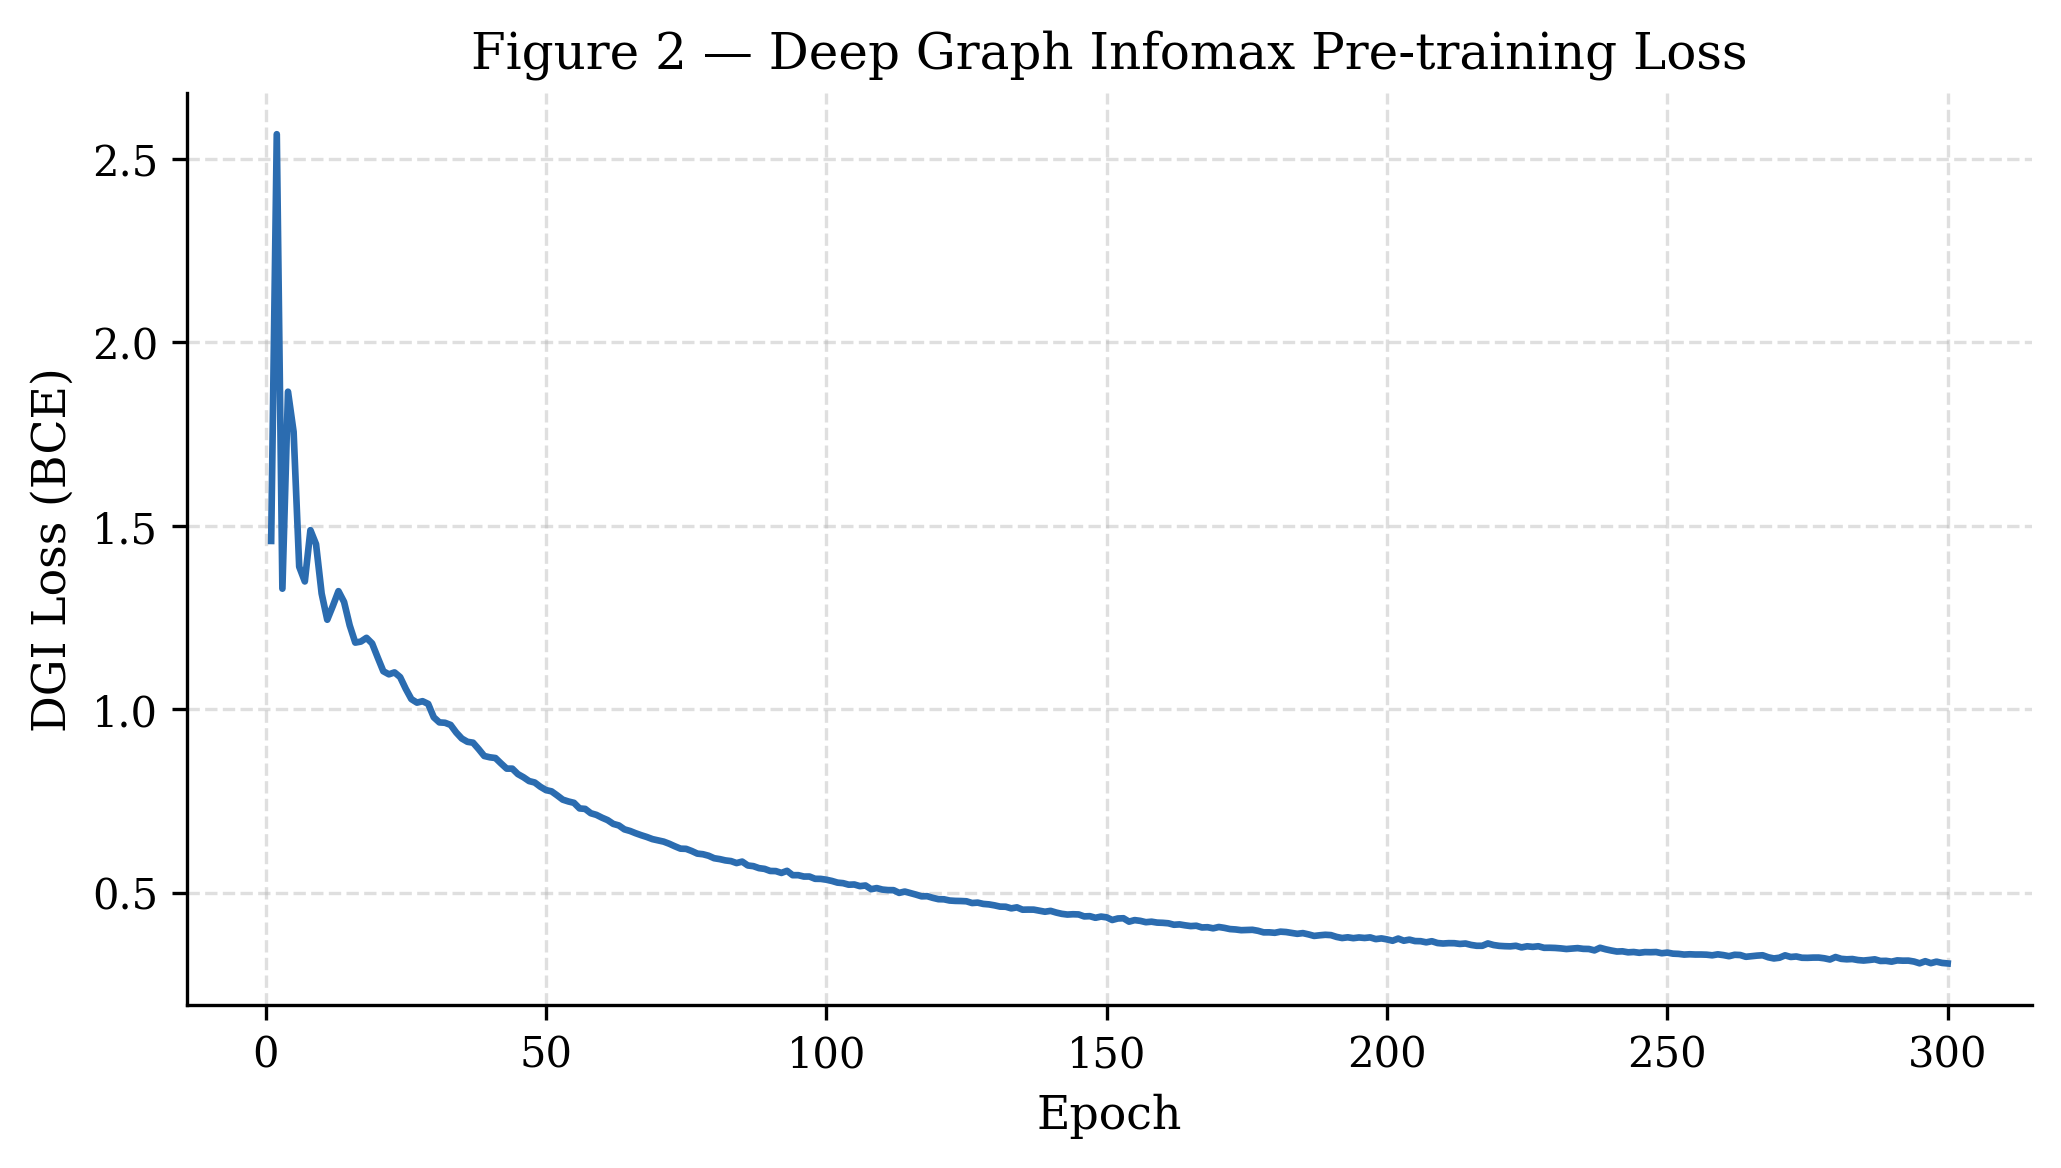
\includegraphics[width=0.75\linewidth]{fig02_dgi_loss.png}
  \caption{DGI training loss over 300 pre-training epochs.
    The binary cross-entropy loss defined in
    Equation~\eqref{eq:dgi} converges from an initial
    value of 1.459 at epoch 1 to stable low values by
    epoch 300, confirming that the encoder successfully
    learns to discriminate real node-summary pairs from
    corrupted pairs across the full 203,769-node graph.}
  \label{fig:dgi_loss}
\end{figure}

\subsubsection{Phase 2: Supervised Graph Attention Network}

The MixTrace GAT architecture~\citep{velickovic2018gat}
processes the full 169-dimensional feature matrix through
two attention layers. The first layer uses eight parallel
attention heads with concatenated outputs; the second
uses a single head. After attention processing, Equation~\eqref{eq:fused}
defines the fused representation that concatenates the GAT
output with the frozen DGI embedding, combining
local attention-derived neighbourhood features with global
topology-derived structural context.

\begin{equation}
  \mathbf{H}_\text{fused}
    = [\mathbf{H}_2 \;\|\; \mathbf{Z}]
    \in \mathbb{R}^{N \times 256},
  \label{eq:fused}
\end{equation}

where $\mathbf{H}_2 \in \mathbb{R}^{N \times 128}$ is the
GAT second-layer output and $\mathbf{Z}$ is the
pre-computed frozen DGI embedding. A two-layer MLP
classifier maps the fused representation to logits
$\hat{\mathbf{y}} \in \mathbb{R}^{N \times 2}$.

\subsubsection{Training Protocol}

Equation~\eqref{eq:loss} defines the class-weighted
cross-entropy loss function, which penalises illicit
misclassifications 4.317 times more heavily than licit
misclassifications to counteract the 9.2:1 imbalance ratio.

\begin{equation}
  \mathcal{L}_\text{GAT}
    = -\sum_{v \in \mathcal{V}_L}
      w_{y_v} \log \hat{p}(y_v \mid v),
  \label{eq:loss}
\end{equation}

where $\mathcal{V}_L$ is the labelled training set,
$w_0 \approx 0.565$ (licit), and $w_1 \approx 4.317$
(illicit). The optimiser is Adam with initial learning
rate $5 \times 10^{-4}$ and weight decay $5 \times 10^{-4}$.
A ReduceLROnPlateau scheduler monitors validation F1
with patience 10 and factor 0.5. Training terminates
after 500 epochs or 20 consecutive epochs without
validation improvement. ADASYN oversampling, following the
density-sensitive synthesis protocol documented
by~\citep{ileberi2024}, was evaluated as an isolated
ablation on the Random Forest baseline rather than folded
into GAT training: ADASYN generates synthetic minority-class
feature vectors that lack a natural position in the
transaction graph, making it structurally awkward to
incorporate into transductive graph training without
introducing disconnected synthetic nodes. Applied instead to
Random Forest on the same tabular features, five-seed
evaluation shows ADASYN oversampling does not improve
illicit-class F1 relative to class-weighted training alone
(0.626 $\pm$ 0.001 with ADASYN versus 0.630 $\pm$ 0.001
without, across the same five seeds), a small but consistent
decrease observed in all five runs. Class-weighted loss
therefore remains the sole imbalance-handling mechanism in
MixTrace's GAT training.

Algorithm~\ref{alg:mixtrace} summarises the complete
MixTrace training and inference procedure, consolidating
the DGI pre-training phase, the supervised GAT phase, and
threshold-calibrated inference into a single unified
specification.

\begin{algorithm}[htbp]
\caption{MixTrace Training and Inference}
\label{alg:mixtrace}
\begin{algorithmic}[1]
\Require Transaction graph
  $\mathcal{G}=(\mathcal{V},\mathcal{E},\mathbf{X})$,
  $\mathbf{X}\in\mathbb{R}^{N\times169}$,
  partial labels $\mathbf{Y}_L$, chronological split
  $\tau_\text{train}\!\in\!\{1,\ldots,34\}$,
  $\tau_\text{val}\!\in\!\{35,\ldots,41\}$,
  $\tau_\text{test}\!\in\!\{42,\ldots,49\}$
\Ensure Predicted labels $\hat{\mathbf{y}}$ for test nodes

\vspace{2pt}
\Statex \textit{Phase 1: DGI Unsupervised Pre-Training}
\For{$\text{epoch} \leftarrow 1$ \textbf{to} $300$}
  \State $\mathbf{H}^{(1)} \leftarrow
    \text{ELU}\!\bigl(\hat{\mathbf{A}}\mathbf{X}\mathbf{W}_1\bigr)
    \in \mathbb{R}^{N\times256}$
    \Comment{GCN layer 1}
  \State $\mathbf{Z} \leftarrow
    \text{ELU}\!\bigl(\hat{\mathbf{A}}\mathbf{H}^{(1)}\mathbf{W}_2\bigr)
    \in \mathbb{R}^{N\times128}$
    \Comment{GCN layer 2}
  \State $\mathbf{s} \leftarrow
    \sigma\!\bigl(\tfrac{1}{N}\textstyle\sum_v\mathbf{z}_v\bigr)$
    \Comment{global graph summary}
  \State $\tilde{\mathbf{X}} \leftarrow \text{shuffle\_rows}(\mathbf{X})$
    \Comment{row-shuffle corruption}
  \State $\tilde{\mathbf{Z}} \leftarrow
    \text{GCN\_encoder}(\tilde{\mathbf{X}})$
  \State Minimise $\mathcal{L}_\text{DGI}$ via Adam
    ($\text{lr}=10^{-3}$,\ $\lambda=5\times10^{-4}$)
\EndFor
\State $\mathbf{Z}^* \leftarrow \mathbf{Z}$
  \Comment{freeze DGI embeddings}

\vspace{2pt}
\Statex \textit{Phase 2: Supervised GAT Training}
\State best\_val\_F1 $\leftarrow 0$;\ no\_improve $\leftarrow 0$
\For{$\text{epoch} \leftarrow 1$ \textbf{to} $500$}
  \State $\mathbf{H}_1 \leftarrow
    \text{GAT}_1(\mathbf{X},\mathbf{A};\;\text{heads}=8)
    \in \mathbb{R}^{N\times128}$
  \State $\mathbf{H}_2 \leftarrow
    \text{GAT}_2(\mathbf{H}_1,\mathbf{A};\;\text{heads}=1)
    \in \mathbb{R}^{N\times128}$
  \State $\mathbf{H}_\text{fused} \leftarrow
    [\mathbf{H}_2 \;\|\; \mathbf{Z}^*]
    \in \mathbb{R}^{N\times256}$
    \Comment{skip connection}
  \State $\hat{\mathbf{y}} \leftarrow
    \text{MLP}(\mathbf{H}_\text{fused})$
  \State Minimise $\mathcal{L}_\text{GAT}$ with
    $w_0\!=\!0.565$, $w_1\!=\!4.317$
    \Comment{class-weighted CE}
  \If{val\_F1 improves}
    \State Save checkpoint;\ best\_val\_F1 $\leftarrow$ val\_F1;\ no\_improve $\leftarrow 0$
  \Else
    \State no\_improve $\leftarrow$ no\_improve $+1$
    \If{no\_improve $\bmod 10 = 0$}
      \State $\text{lr} \leftarrow \text{lr} \times 0.5$
        \Comment{ReduceLROnPlateau, factor 0.5}
    \EndIf
    \If{no\_improve $\geq 20$}
      \textbf{ break}
    \EndIf
  \EndIf
\EndFor
\State Load best checkpoint $\boldsymbol{\theta}^*$

\vspace{2pt}
\Statex \textit{Inference}
\State $\hat{p} \leftarrow
  \sigma\!\bigl(\text{MLP}_{\boldsymbol{\theta}^*}(
    [\text{GAT}(\mathbf{X}_\text{test})\,\|\,
     \mathbf{Z}^*_\text{test}])\bigr)$
\State $\theta^* \leftarrow \arg\max_\theta
  F_1(\hat{p} \geq \theta,\;\mathbf{Y}_\text{val})$
  \Comment{$\theta^*\!=\!0.9397$}
\State $\hat{\mathbf{y}} \leftarrow
  \mathbf{1}[\hat{p} \geq \theta^*]$
\State \Return $\hat{\mathbf{y}}$
\end{algorithmic}
\end{algorithm}

% ─────────────────────────────────────────────────────────────
\section{Experiments}
\label{sec:exp}
% ─────────────────────────────────────────────────────────────

\subsection{Datasets}
\label{sec:data}

\paragraph{Elliptic Bitcoin Dataset.}
The Elliptic dataset~\citep{weber2019} comprises 203,769
Bitcoin transaction nodes across 49 weekly time steps with
165 features: 93 local transaction features and 72
aggregated one-hop neighbourhood features. Class
distribution among 46,564 labelled nodes is 4,545 illicit
(9.76 percent) and 42,019 licit (90.24 percent), yielding
a 9.2:1 imbalance ratio. A strict chronological split
assigns time steps 1 to 34 to training (136,265 nodes),
35 to 41 to validation (30,680 nodes), and 42 to 49 to
the held-out test set (36,824 nodes), preventing temporal
data leakage. The test partition contains 408 illicit
and 8,433 licit labelled nodes. Structural analysis of this
dataset family, including its extended version, has been
conducted by~\citet{bellei2024}.

Figure~\ref{fig:class_dist} plots the class distribution
across labelled nodes in the Elliptic Bitcoin Dataset: the
severe 9.2:1 licit-to-illicit imbalance motivates the
class-weighted loss function and ADASYN diagnostic
implemented in the MixTrace pipeline.
\begin{figure}[htbp]
  \centering
  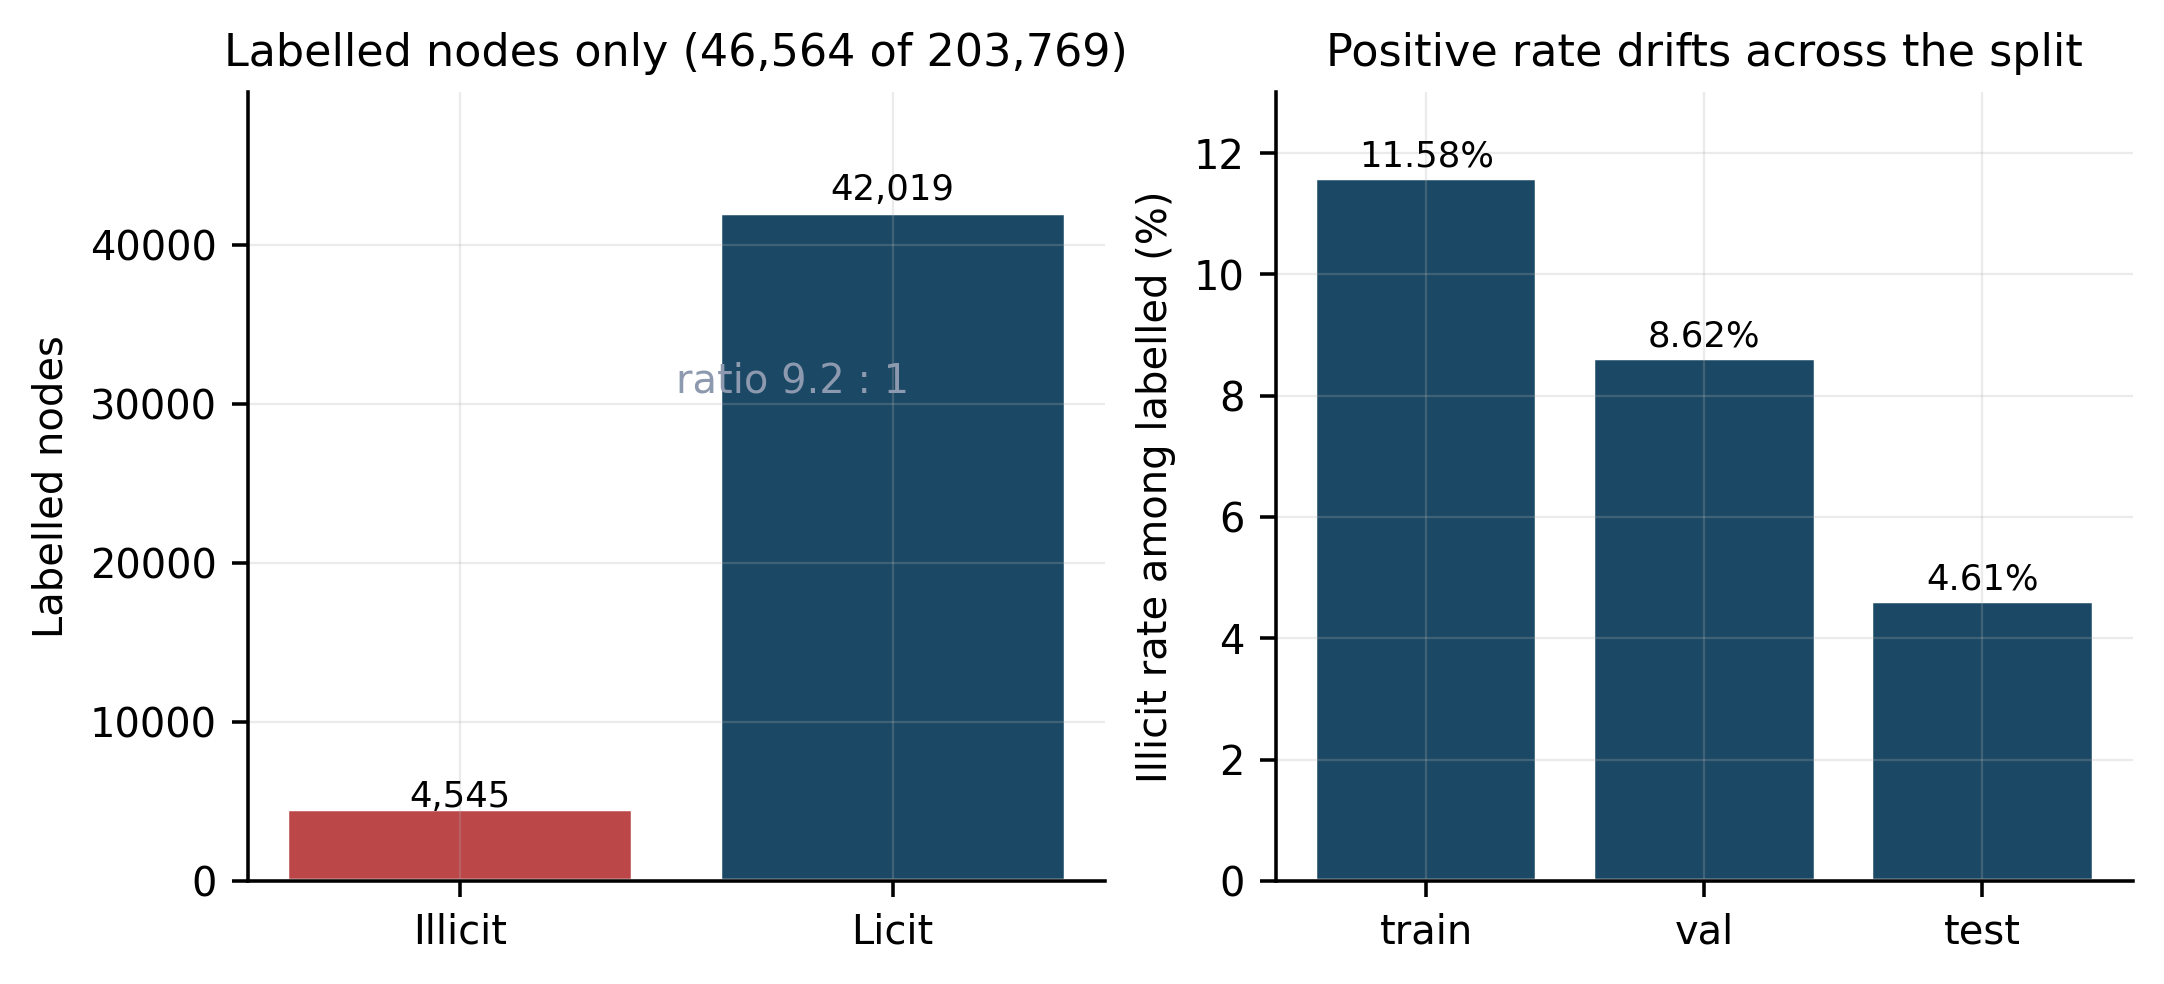
\includegraphics[width=0.92\linewidth]{fig_class_distribution.png}
  \caption{Class composition of the Elliptic Data Set. The left
    panel shows only the 46,564 labelled nodes, 4,545 illicit
    and 42,019 licit, giving a licit-to-illicit ratio of 9.2 to
    1; the 157,205 unlabelled nodes are excluded from the panel
    and from every loss and metric, and take part solely in
    message passing. An earlier version of this figure plotted
    unlabelled nodes alongside a caption describing labelled
    nodes, and the inconsistency is corrected here. The right
    panel shows that the illicit rate among labelled nodes falls
    from 11.58 percent in the training period to 8.62 percent in
    validation and 4.62 percent in test, so the class balance is
    not stationary across the chronological split.}
  \label{fig:class_dist}
\end{figure}

\paragraph{Author-Curated Bitcoin Transaction Corpus.}
A corpus of 5,884,387 Bitcoin transactions with 53
engineered features including script-type indicators,
fee rates, input and output counts, address-reuse flags,
and value metrics was assembled. The ground-truth label
\texttt{is\_coinjoin\_like} identifies 110,352 transactions
(1.88 percent) as screening candidates. Section~\ref{sec:screening}
establishes that the field is the deterministic rule in
Equation~\eqref{eq:cjrule} rather than a heuristic validated
against known mixing services, and the earlier description is
corrected accordingly.

\paragraph{Correction to the reported script coverage.}
An earlier version of the present study reported that the corpus
predates widespread Pay-to-Taproot adoption and contains zero
confirmed P2TR transactions, and structural clustering was
therefore conducted on multi-input P2WPKH proxies. That statement
was incorrect, and the correction matters because it removes the
principal limitation previously attached to the clustering
analysis.

The corpus carries six boolean script-type indicators, covering
P2PK, P2PKH, P2SH, P2WPKH, P2WSH and Taproot. Every one of the
six is \texttt{False} for every one of the 5{,}884{,}387 rows, so
no script type could be confirmed through them, and the absence
of confirmed Taproot was an artefact of the indicator columns
rather than a property of the data. Script information is in fact
present in the corpus, in the \texttt{input\_script\_types} and
\texttt{output\_script\_types} fields, which carry the script
descriptors reported by the node.

Parsing those descriptors gives the composition in
Table~\ref{tab:script_composition}. Taproot accounts for 24.10
percent of outputs; 2{,}494{,}168 transactions, or 42.39 percent
of the corpus, involve a Taproot script on at least one side; and
among the 110,352 screening candidates the proportion rises to
71.94 percent. The corpus spans 13 July 2022 to 1 July 2025,
beginning roughly eight months after Taproot activation at block
709{,}632, and is post-Taproot throughout.

\begin{table}[htbp]
\centering
\small
\caption{Output script composition of the author-curated corpus,
reconstructed from node-reported script descriptors after the six
distributed indicator columns were found to be uniformly false.}
\label{tab:script_composition}
\begin{tabular}{lr}
\toprule
Output script type & Share of outputs \
\midrule
P2WPKH (\texttt{witness\_v0\_keyhash})        & 38.66\,\% \
\textbf{P2TR (\texttt{witness\_v1\_taproot})} & \textbf{24.10\,\%} \
P2SH (\texttt{scripthash})                    & 15.61\,\% \
P2PKH (\texttt{pubkeyhash})                   & 12.39\,\% \
OP\_RETURN (\texttt{nulldata})                &  6.84\,\% \
P2WSH (\texttt{witness\_v0\_scripthash})      &  2.25\,\% \
Bare multisig                                 &  0.15\,\% \
\bottomrule
\end{tabular}
\end{table}

The P2WPKH proxy is therefore unnecessary, and the claims made
for script-agnostic structural screening are supported by direct
measurement on post-Taproot data rather than by extrapolation
from a pre-Taproot substitute.

\subsection{Baseline Methods}

\textbf{K-Means} ($k=2$) applies Euclidean clustering to
the standardised node feature matrix with cluster-to-class
assignment via majority vote over training labels.

\textbf{K-Nearest Neighbours (KNN)} applies grid search
over $k \in \{3,5,7,11,15\}$ and uniform/distance
weighting, selecting the configuration maximising
validation illicit F1.

\textbf{Random Forest (RF)} applies grid search over
estimator count in $\{100,200\}$, maximum depth in
$\{10,20,\text{None}\}$, and minimum split samples in
$\{2,5\}$ with balanced class weighting.

\textbf{GAT without DGI} is a dedicated architecture with
its own 128-dimensional GAT output feeding directly into a
correspondingly sized MLP head, trained end-to-end from
epoch 1 with no DGI-derived input at any stage. This
supersedes an earlier ablation design that reused the
fully DGI-trained MixTrace model and zeroed its DGI skip
connection only at inference time; that design measured
the effect of removing DGI information from an already
DGI-adapted classifier rather than the effect of never
having DGI available during training, and its results are
retained only in the single-run illustrative figures of
Section~\ref{sec:class_results} for continuity with the
original exploratory analysis. The dedicated architecture
isolates the DGI contribution while preserving attention
layer structure and hyperparameters, consistent with
ablation methodology recommended by~\citet{motie2024}, and
removes the zero-padding approximation entirely: every
weight in the ablation model is trained against a genuinely
DGI-free objective from initialisation.

\subsection{Illicit Transaction Detection Results}
\label{sec:class_results}

Table~\ref{tab:classification} presents test-set classification
performance for all evaluated methods on the Elliptic held-out
partition containing 408 illicit and 8,433 licit labelled nodes,
aggregated as mean $\pm$ standard deviation across five
independent random seeds (1, 2, 3, 42, 123). For each seed, the
DGI encoder, the MixTrace GAT, and the GAT-without-DGI ablation
were retrained from scratch; K-Means, KNN, and Random Forest
were correspondingly refitted. The GAT-without-DGI ablation is
a genuinely separate model trained end-to-end with the DGI skip
connection replaced by a zero tensor from epoch 1 onward, rather
than a single DGI-equipped model evaluated with its skip input
zeroed only at test time.

\begin{table}[htbp]
  \caption{Illicit transaction detection results on the
    Elliptic test set (time steps 42--49), reporting
    precision, recall, illicit F1, macro F1, PR-AUC, and
    ROC-AUC for all methods as mean $\pm$ standard deviation
    across five random seeds (1, 2, 3, 42, 123). Best result
    per column appears in \textbf{bold}; K-Means' trivial
    recall of 1.000 reflects an all-positive degenerate
    classifier and is excluded from bolding on that basis.}
  \label{tab:classification}
  \centering
  \scriptsize
  \setlength{\tabcolsep}{3.5pt}
  \begin{tabular}{lcccccc}
    \toprule
    \textbf{Method}
      & \textbf{Prec.} & \textbf{Rec.}
      & \textbf{F1} & \textbf{F1\textsubscript{mac}}
      & \textbf{PR-AUC} & \textbf{ROC-AUC} \\
    \midrule
    K-Means
      & 0.047$\pm$.002 & 1.000$\pm$.000 & 0.090$\pm$.003 & 0.070$\pm$.034 & 0.000$\pm$.000 & -- \\
    KNN
      & 0.510$\pm$.000 & 0.456$\pm$.000 & 0.481$\pm$.000 & 0.729$\pm$.000 & 0.447$\pm$.000 & 0.794$\pm$.000 \\
    Random Forest
      & \textbf{0.954$\pm$.005} & 0.470$\pm$.001 & 0.630$\pm$.001 & 0.808$\pm$.001 & 0.640$\pm$.004 & 0.937$\pm$.002 \\
    GAT (no DGI, retrained)
      & 0.377$\pm$.234 & 0.878$\pm$.101 & 0.482$\pm$.205 & 0.705$\pm$.134 & 0.813$\pm$.037 & 0.961$\pm$.021 \\
    \textbf{MixTrace (DGI+GAT)}
      & 0.713$\pm$.115 & \textbf{0.934$\pm$.047} & \textbf{0.806$\pm$.090} & \textbf{0.897$\pm$.048}
      & \textbf{0.862$\pm$.124} & \textbf{0.992$\pm$.005} \\
    \bottomrule
  \end{tabular}
\end{table}

MixTrace achieves the highest mean illicit F1-score (0.806),
macro F1 (0.897), PR-AUC (0.862), and ROC-AUC (0.992) across
the five seeds.
Random Forest attains the highest precision (0.954) at the
cost of recall (0.470). The retrained standalone GAT without
DGI shows high-recall, low-precision behaviour on average
(recall 0.878, precision 0.377, F1 0.482) with substantial
across-seed variability (F1 standard deviation 0.205, versus
0.090 for MixTrace), confirming that
graph attention layers alone collapse toward near-unconditional
positive prediction without structural pre-training context
under the 9.2:1 imbalance ratio~\citep{alarab2024}.

Figures~\ref{fig:pr_curves}--\ref{fig:confusion} illustrate
curve- and matrix-level behaviour for a single representative
seed rather than the five-seed aggregate; the corresponding
GAT-without-DGI curves reflect the original single-run ablation
protocol (DGI skip zeroed only at inference on an already-DGI-trained
model) that Table~\ref{tab:classification} supersedes with a
properly retrained ablation, so the exact values below should
not be read as the paper's headline multi-seed statistics.
Figure~\ref{fig:pr_curves} plots the precision-recall curves
for all methods on that representative run: MixTrace maintains
superior precision across
the full recall spectrum compared to all baselines.
Figure~\ref{fig:roc_curves} presents the corresponding ROC
curves for the same run, illustrating MixTrace's ranking
quality.

\begin{figure}[htbp]
  \centering
  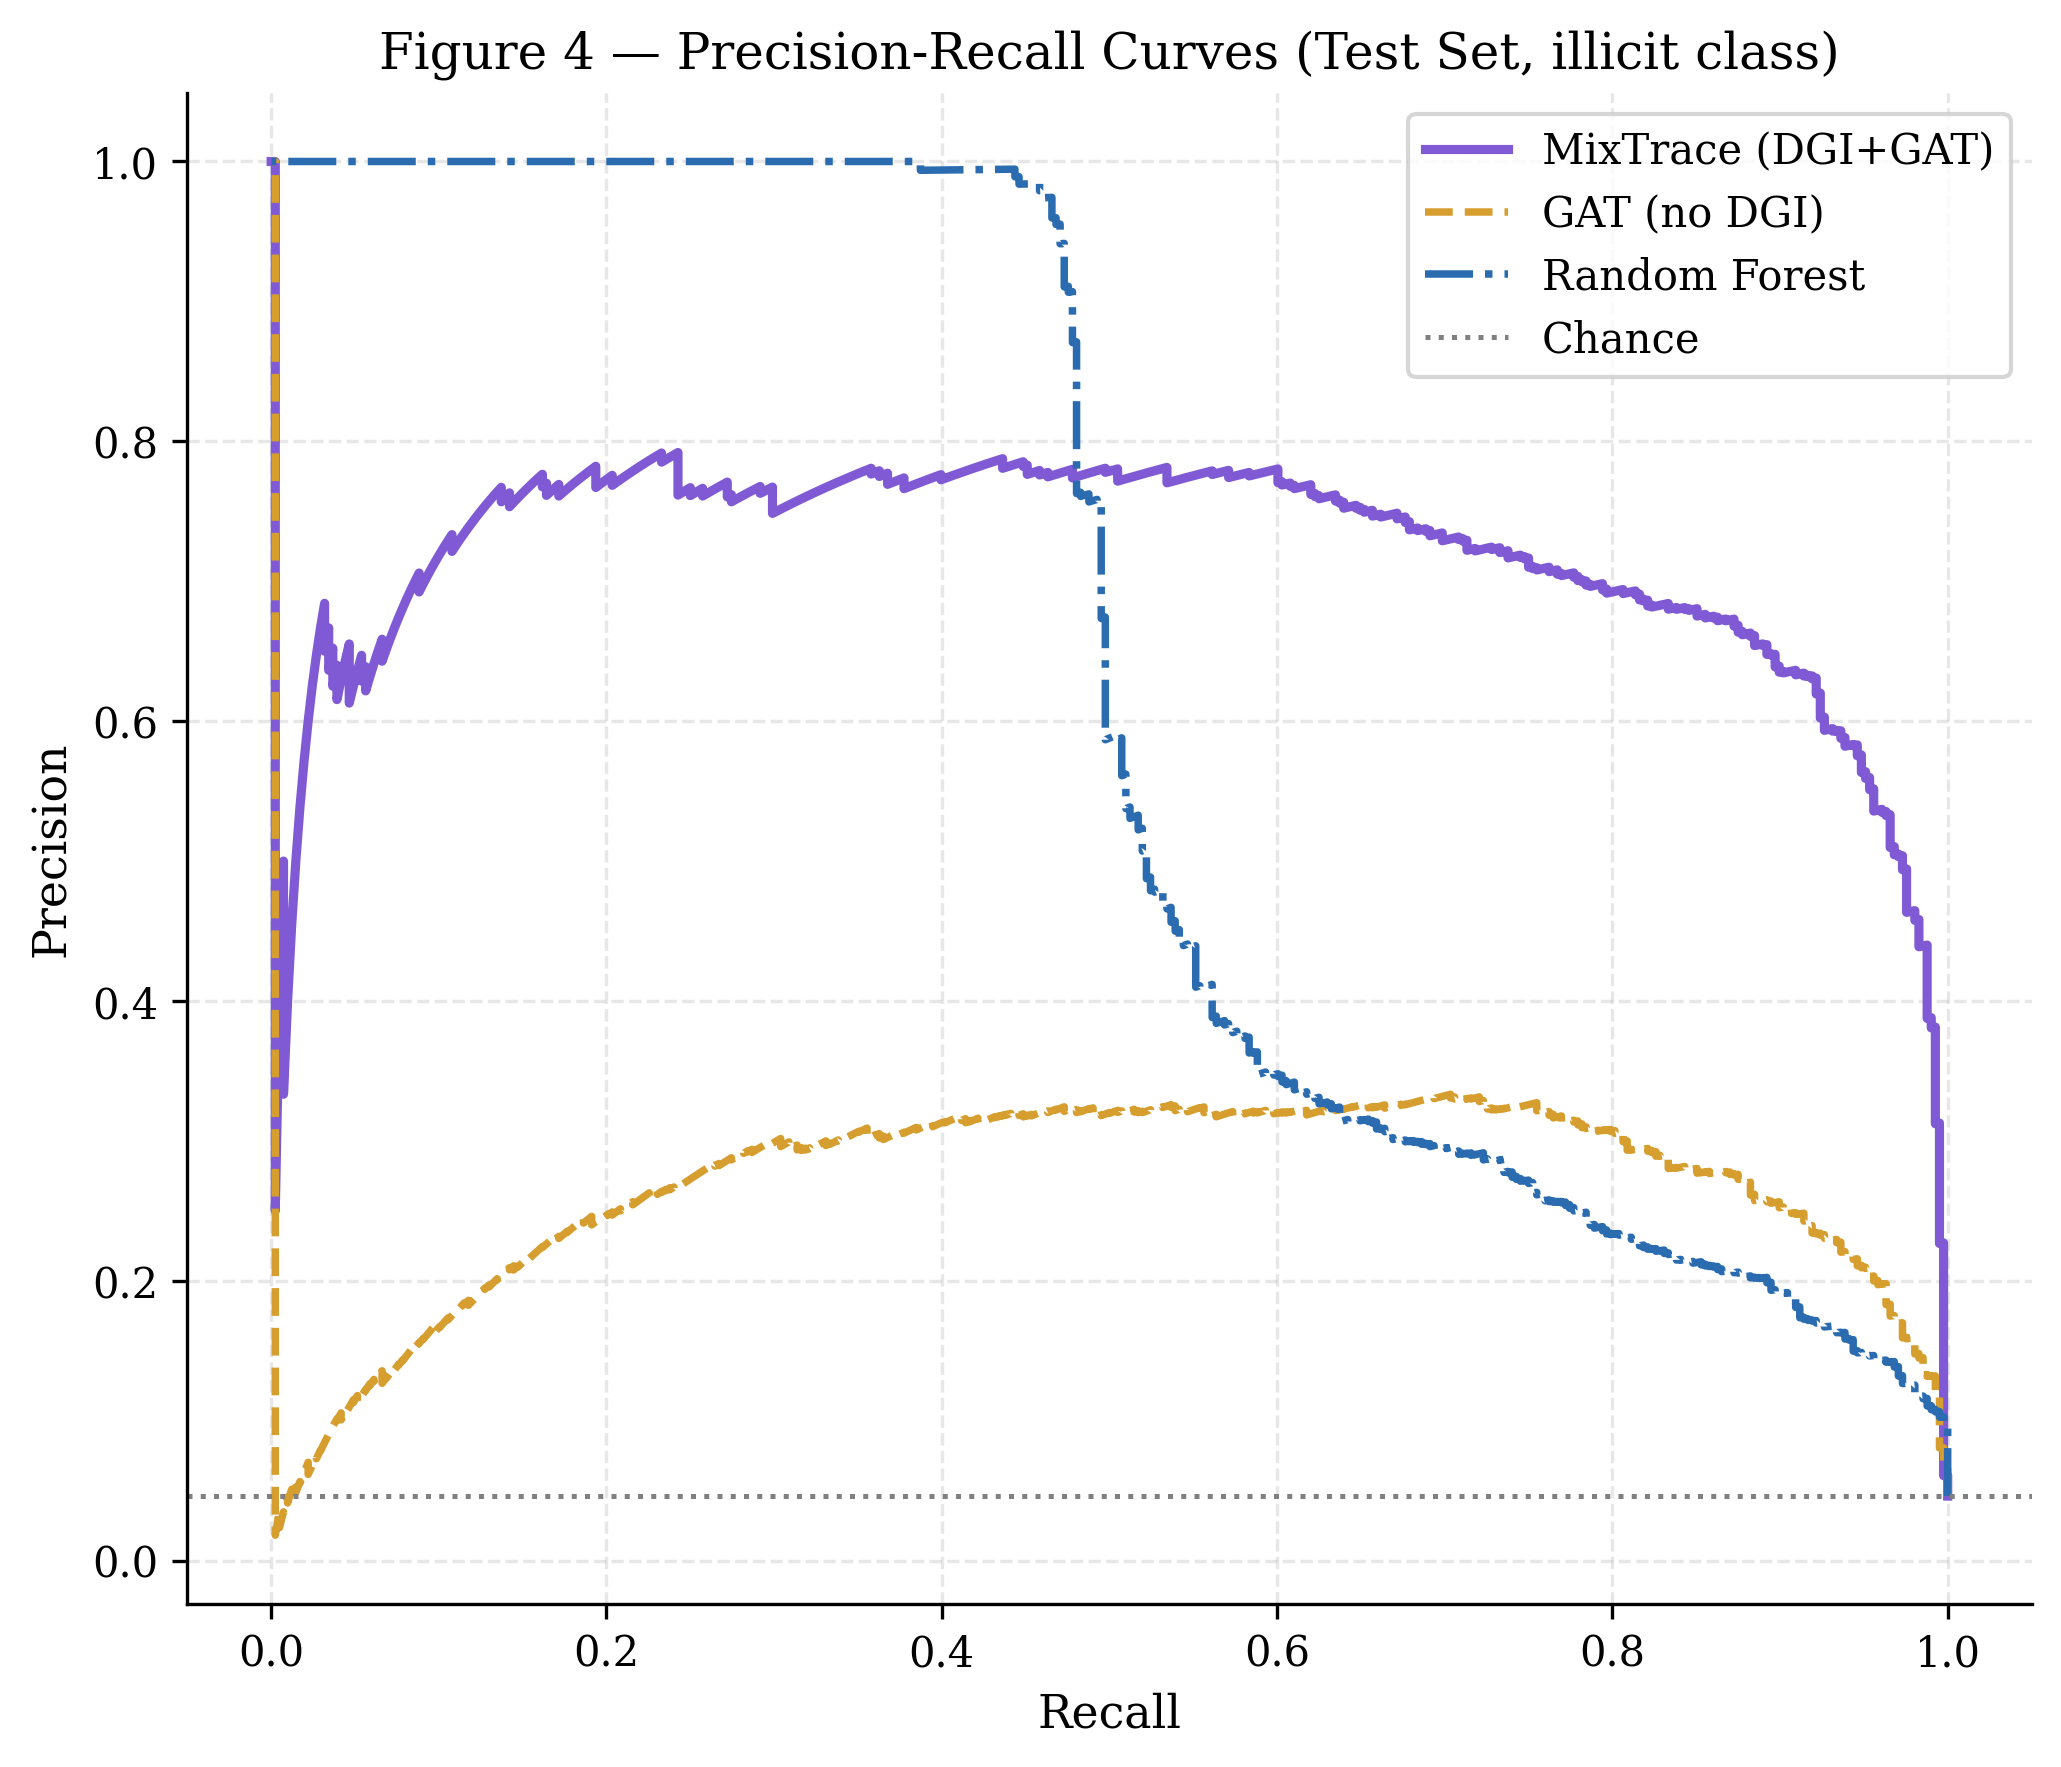
\includegraphics[width=0.85\linewidth]{fig04_pr_curves.png}
  \caption{\textbf{Single representative run (seed 42); see
    Table~\ref{tab:classification} for the five-seed mean
    $\pm$ standard deviation.} Precision-recall curves for all evaluated methods
    on the Elliptic test set. MixTrace (DGI+GAT) maintains
    substantially higher precision across the full range of
    recall values compared to all baseline methods, with a
    PR-AUC of 0.7167 versus 0.6316 for the best competing
    method (Random Forest) in this run, reflecting superior
    ranking quality of illicit-class probability scores.}
  \label{fig:pr_curves}
\end{figure}

\begin{figure}[htbp]
  \centering
  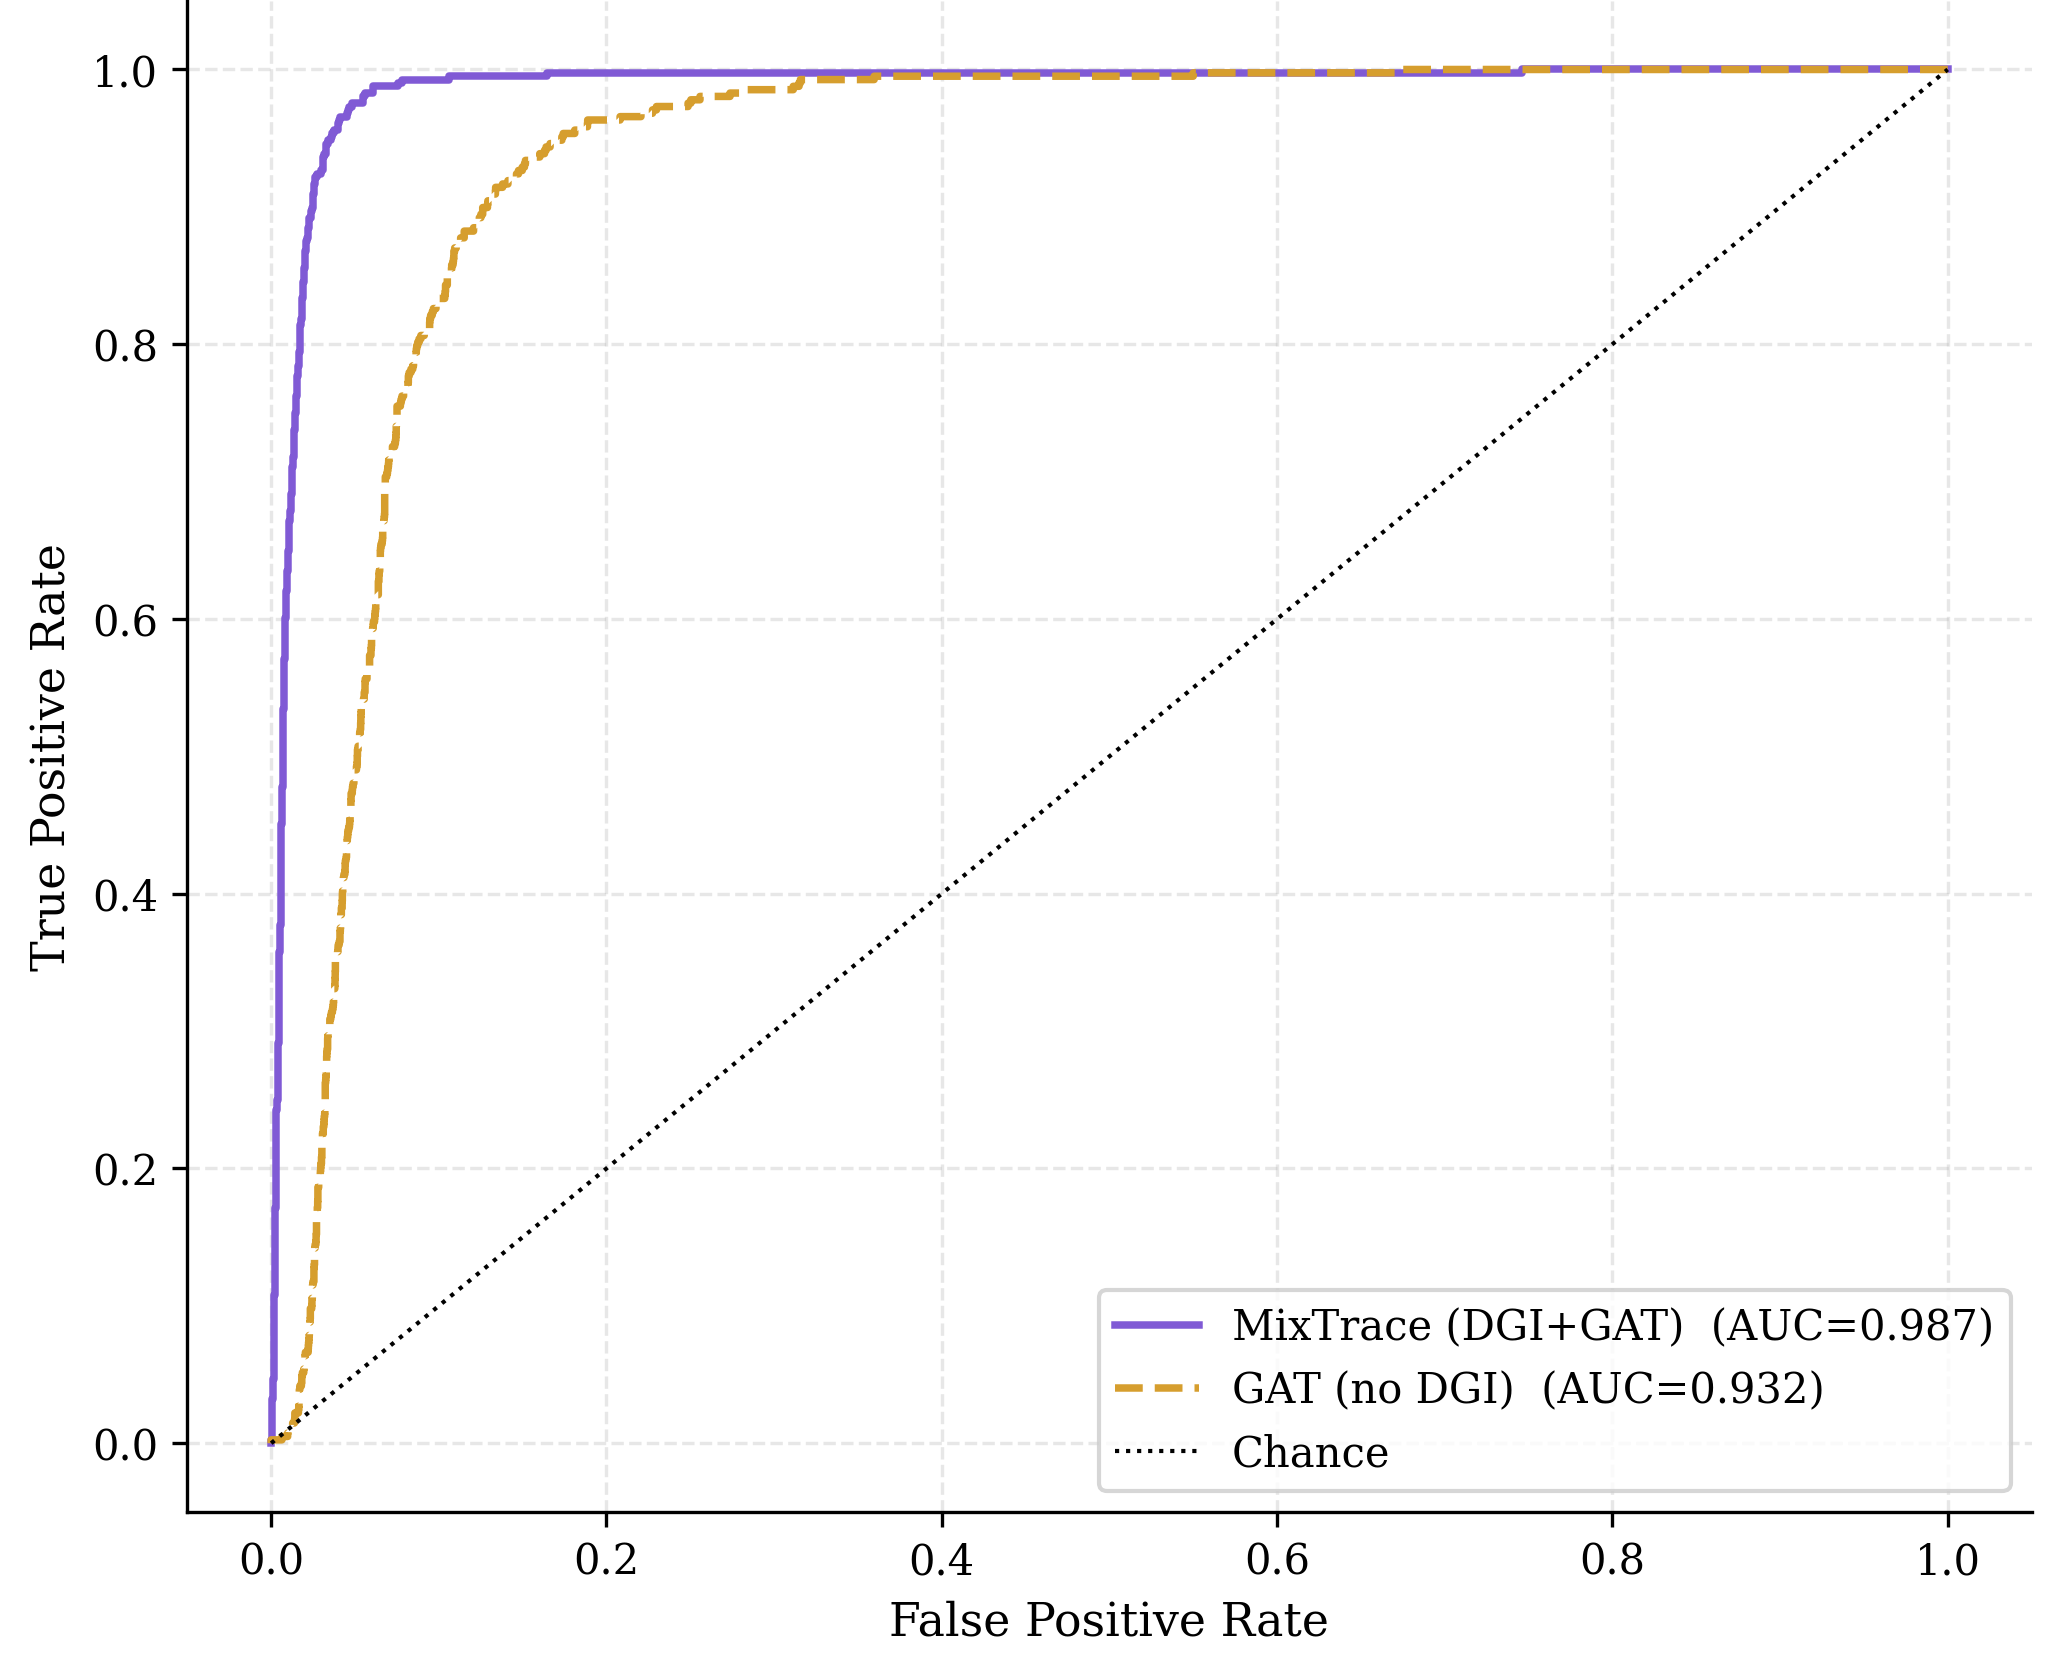
\includegraphics[width=0.85\linewidth]{fig05_roc_curves.png}
  \caption{\textbf{Single representative run (seed 42), same
    run as Figure~\ref{fig:pr_curves}; see
    Table~\ref{tab:classification} for the five-seed mean
    $\pm$ standard deviation.} Receiver operating characteristic curves for all
    evaluated methods. MixTrace achieves the highest area
    under the ROC curve (0.9868 in this run) among all evaluated
    approaches; the GAT trained under the original single-run
    ablation protocol (DGI skip zeroed only at inference) attains a lower ROC-AUC
    of 0.9319 despite its high raw recall. The properly
    retrained GAT-without-DGI ablation of
    Table~\ref{tab:classification} tells a fuller story:
    mean ROC-AUC of 0.961 with substantially higher variance
    than MixTrace across seeds.}
  \label{fig:roc_curves}
\end{figure}

Figure~\ref{fig:confusion} presents the confusion matrices for
all five evaluated methods on that same representative run,
laying out the decision-boundary
characteristics of each approach and the transition from the
degenerate all-positive patterns of K-Means and
the original single-run GAT-without-DGI ablation to the balanced true-positive/true-negative
performance of MixTrace.

\begin{figure}[htbp]
  \centering
  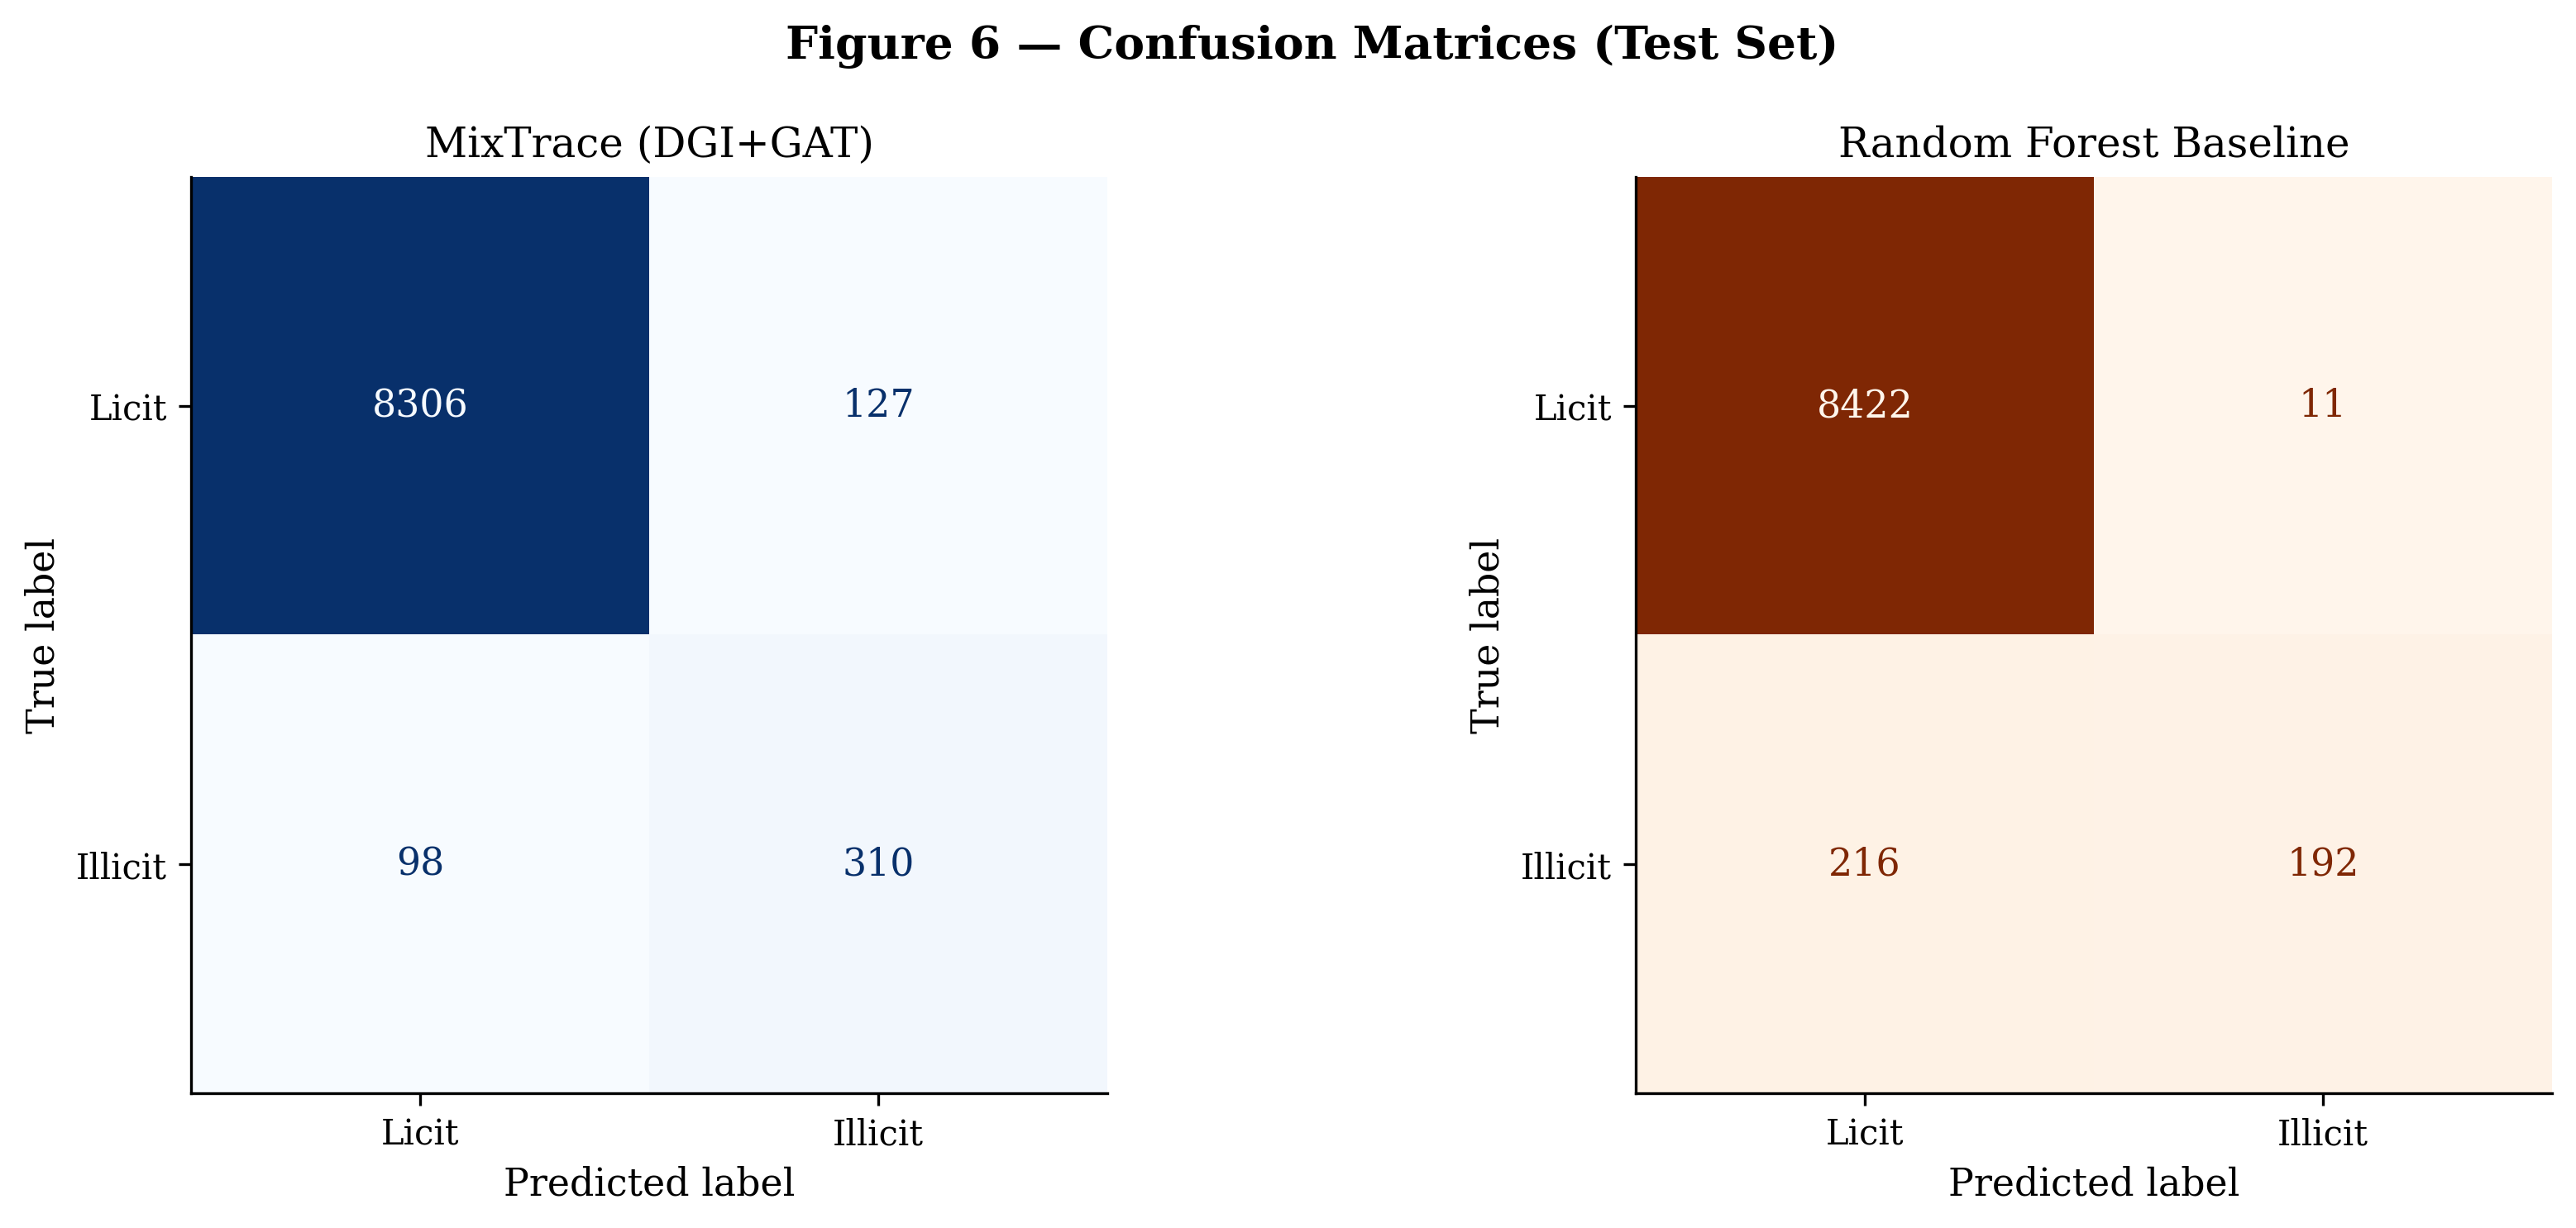
\includegraphics[width=\linewidth]{fig06_confusion_matrices.png}
  \caption{\textbf{Single representative run (seed 42); see
    Table~\ref{tab:classification} for the five-seed mean
    $\pm$ standard deviation.} Confusion matrices for all evaluated methods on
    the Elliptic test set (408 illicit, 8,433 licit nodes).
    The progression runs from degenerate all-positive
    prediction in K-Means (22 TN, 8,433 FP) and the original
    single-run GAT-without-DGI ablation, through the high-precision but low-recall behaviour
    of Random Forest, to the balanced classification of
    MixTrace with 310 TP, 8,306 TN, 98 FN, and 127 FP
    (precision $= 310/437 = 0.709$) in this run.}
  \label{fig:confusion}
\end{figure}

\subsection{Self-Supervised Pre-Training and Supervised Training Dynamics}

This subsection describes epoch-level training dynamics for
the original single representative seed used to generate
Figure~\ref{fig:training_curves}; Table~\ref{tab:classification}
and Table~\ref{tab:stats} report the aggregate five-seed
statistics. The DGI encoder was pre-trained for 300 epochs. Initial
loss at epoch 1 was 1.459, reflecting random encoder
weights. Supervised GAT training began at learning rate
$5 \times 10^{-4}$. At epoch 5, training F1 reached 0.8423
and validation F1 reached 0.5094. By epoch 20, training F1
improved to 0.8844 and validation F1 to 0.5847. Convergence
stabilised between epochs 220 and 265, where training F1
exceeded 0.9550 and the best validation macro F1 of 0.8864
was recorded at epoch 235. The optimal decision threshold
was $\theta^* = 0.9397$.

Figure~\ref{fig:training_curves} traces the training and
validation F1-score curves across supervised training epochs: both
improve steadily, confirming stable convergence without
overfitting under early stopping.

\begin{figure}[htbp]
  \centering
  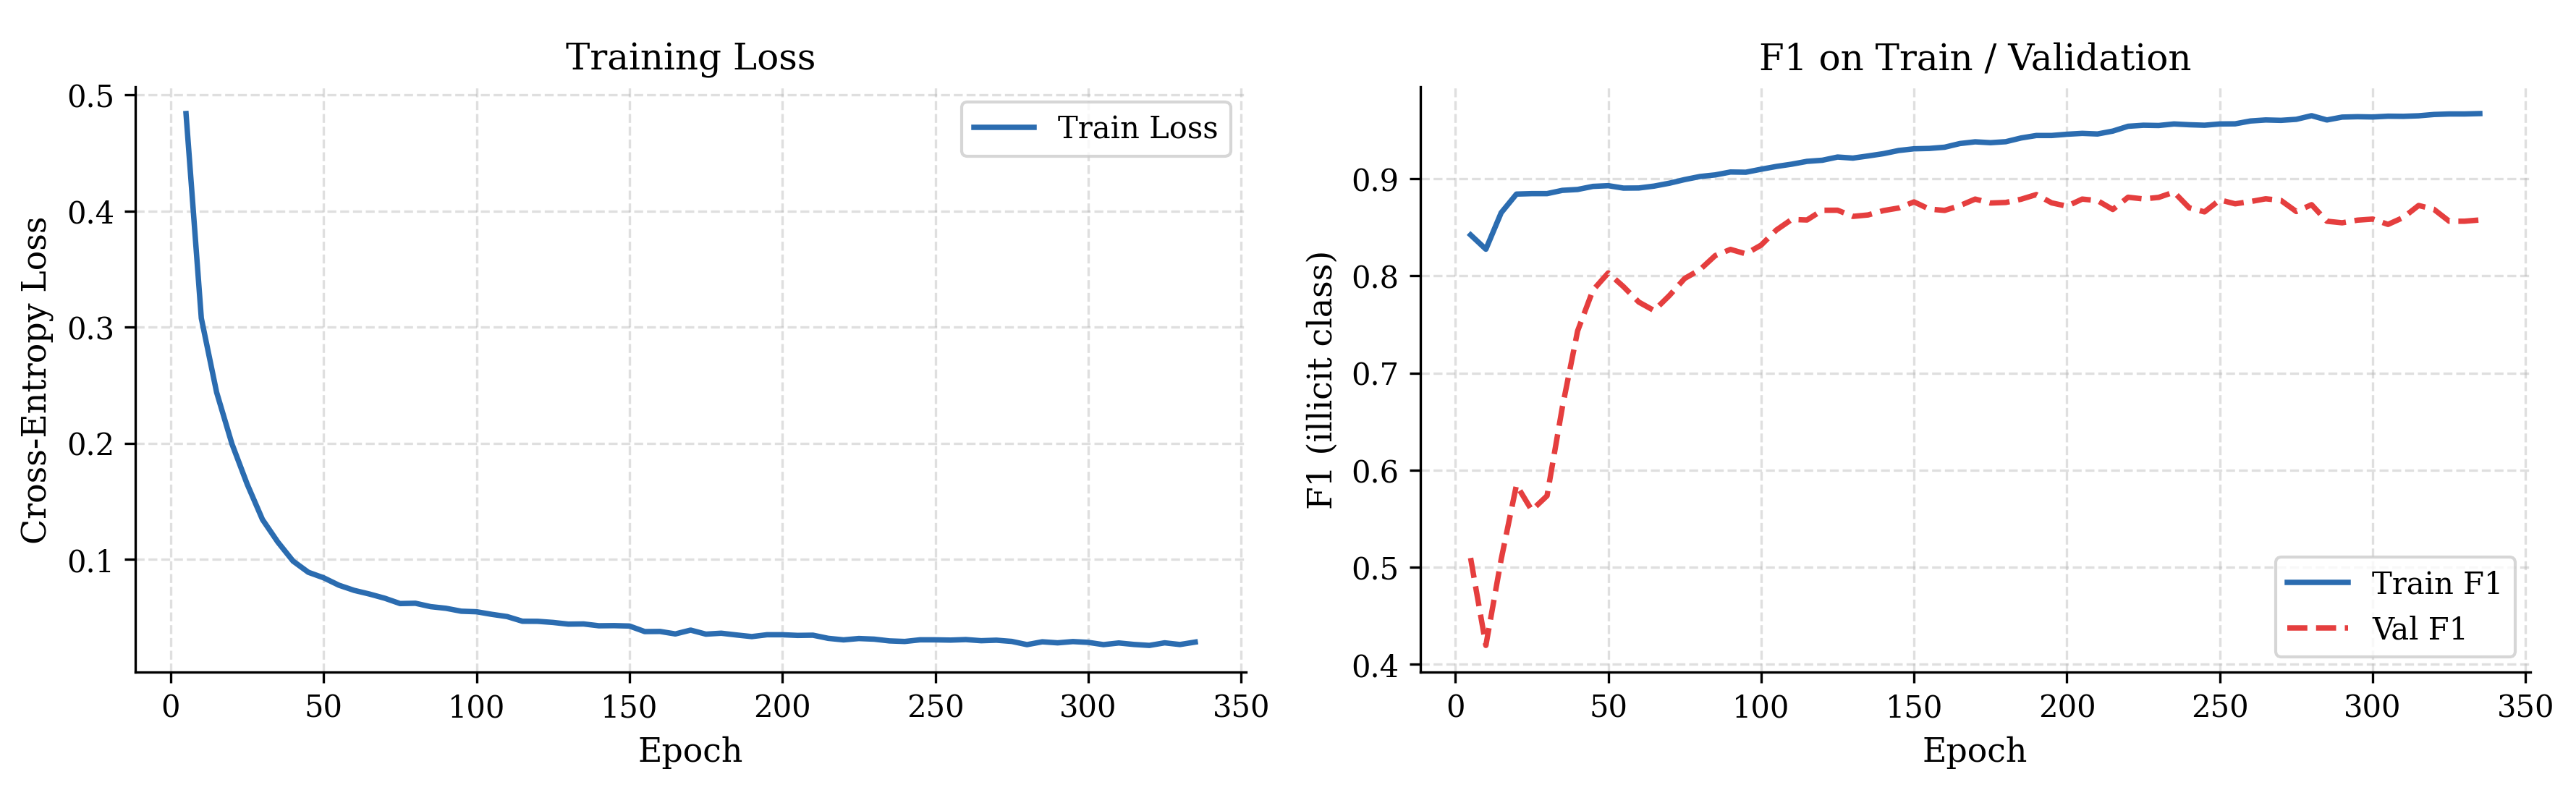
\includegraphics[width=0.85\linewidth]{fig07_training_curves.png}
  \caption{\textbf{Single representative run (seed 42).} Supervised GAT training curves showing training
    F1-score, validation F1-score, and learning rate
    schedule across supervised training epochs. Both metrics follow
    a consistent upward trajectory, training reaching 0.9550
    by epoch 220 and validation reaching a best macro F1 of
    0.8864 at epoch 235, with the learning rate reduction
    triggered by ReduceLROnPlateau visible as step decreases
    at plateau epochs.}
  \label{fig:training_curves}
\end{figure}

Figure~\ref{fig:tsne} plots the t-SNE embeddings of the
pre-trained DGI node representations, coloured by class
label. Illicit nodes (red) cluster into geometrically
distinct regions of the 128-dimensional embedding space,
confirming that the unsupervised DGI pre-training on all
203,769 nodes learns a latent representation that separates
illicit from licit transaction topology even before
supervised training.

\begin{figure}[htbp]
  \centering
  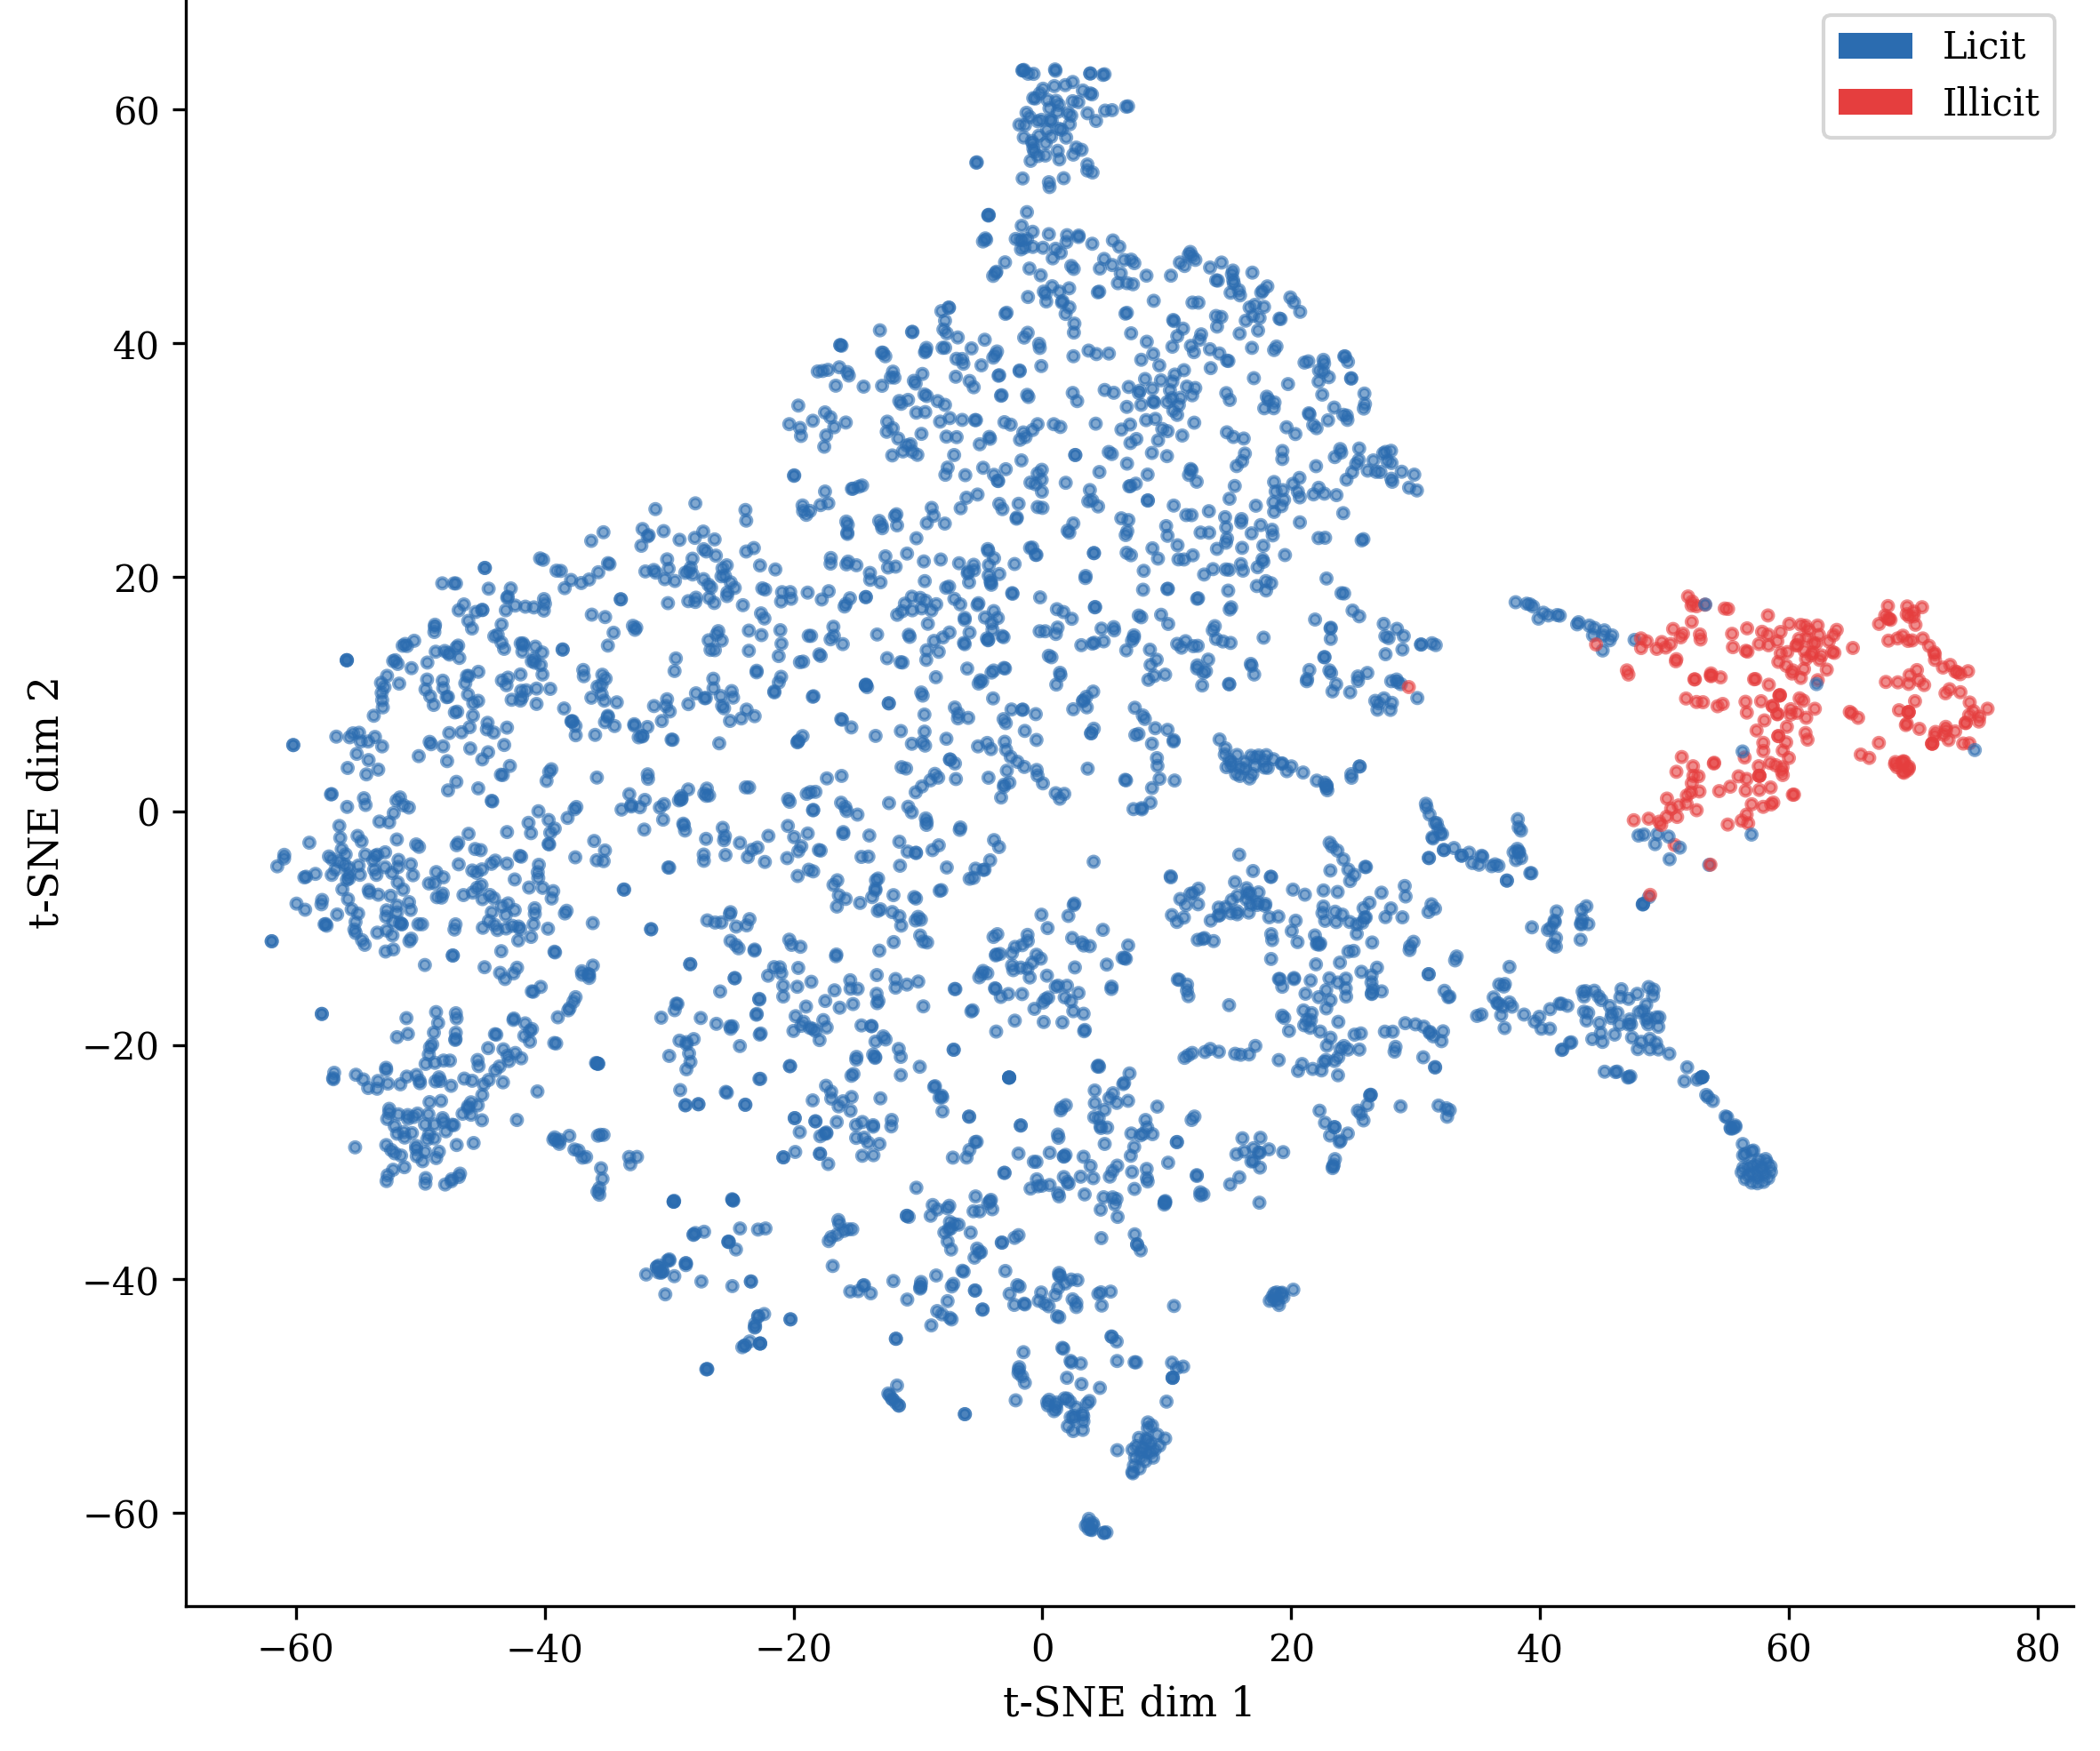
\includegraphics[width=0.80\linewidth]{fig08_tsne_embeddings.png}
  \caption{Two-dimensional t-SNE projection of the
    128-dimensional DGI pre-trained node embeddings,
    coloured by class label (red: illicit, blue: licit,
    grey: unknown). Illicit nodes occupy geometrically
    distinct cluster regions in the learned embedding space,
    confirming that self-supervised DGI pre-training on the
    full 203,769-node graph captures latent structural
    patterns predictive of illicit activity before any
    supervised labels are used.}
  \label{fig:tsne}
\end{figure}

\subsection{Temporal Behaviour and the Marketplace Shock}
\label{sec:temporal_drift}

Round-1 reported a single pooled figure over the test window.
Broken out by time step, as requested during review, performance
proves to be bimodal rather than gradually degrading, and the
pooled figure describes no part of the window well.

\subsubsection{Protocol Comparison}

Before interpreting the breakdown it is necessary to establish
that the leakage-free baseline is sound rather than weak.
Table~\ref{tab:protocol_comparison} evaluates the same learner
under two evaluation windows: the window used in the present
study, and the window adopted in the wider Elliptic literature.
Because a threshold may never be drawn from the test split, the
literature window reserves the final part of the training period
for threshold selection.

\begin{table}[htbp]
\centering
\small
\caption{The same Random Forest on the 165 distributed features
under two evaluation windows, mean over five seeds. The
literature window is consistent with published figures for this
learner, which establishes that the lower value under the present
window is a property of the window rather than of the baseline.}
\label{tab:protocol_comparison}
\begin{tabular}{lcccccc}
\toprule
Evaluation window & F1 & Precision & Recall & PR-AUC & ROC-AUC & MCC \
\midrule
Steps 42--49 (present study) & 0.6212 & 0.9231 & 0.4681 & 0.5431 & 0.8470 & 0.6470 \
Steps 35--49 (literature)    & 0.7634 & 0.8114 & 0.7224 & 0.7813 & 0.9128 & 0.7498 \
\bottomrule
\end{tabular}
\end{table}

\subsubsection{Per-Step Breakdown}

Figure~\ref{fig:temporal_collapse} and
Table~\ref{tab:per_timestep} give the breakdown. Through time
step 42 the classifier is strong, with a mean illicit-class
F1-score of 0.8582 and mean recall of 0.8497. At step 43 recall
falls from 0.789 to zero and does not recover, and the mean
F1-score across the remaining steps is 0.0283. The discontinuity
coincides with the closure of a major darknet marketplace, an
event documented in the dataset's accompanying literature, after
which the illicit population is generated by a different process
from the one the classifier was fitted to.

\begin{table}[htbp]
\centering
\small
\caption{Per-time-step test performance under the literature
window, mean over five seeds, at a threshold selected on
validation and frozen. Performance is bimodal about step 43.}
\label{tab:per_timestep}
\begin{tabular}{rrrcccc}
\toprule
Step & Nodes & Illicit & F1 & Precision & Recall & ROC-AUC \
\midrule
35 & 1{,}341 & 182 & 0.9566 & 0.9465 & 0.9670 & 0.9956 \
36 & 1{,}708 &  33 & 0.7991 & 0.6691 & 1.0000 & 0.9998 \
37 &    498  &  40 & 0.7666 & 0.9926 & 0.6250 & 0.9156 \
38 &    756  & 111 & 0.9210 & 0.9401 & 0.9027 & 0.9637 \
39 & 1{,}183 &  81 & 0.8876 & 0.8540 & 0.9259 & 0.9876 \
40 & 1{,}211 & 112 & 0.7388 & 0.8466 & 0.6571 & 0.8922 \
41 & 1{,}132 & 116 & 0.9425 & 0.9546 & 0.9310 & 0.9829 \
42 & 2{,}154 & 239 & 0.8535 & 0.9298 & 0.7891 & 0.9529 \
\midrule
\textbf{43} & 1{,}370 & 24 & \textbf{0.0000} & 0.0000 & \textbf{0.0000} & 0.7909 \
44 & 1{,}591 & 24 & 0.0316 & 0.0269 & 0.0417 & 0.6852 \
45 & 1{,}221 &  5 & 0.0000 & 0.0000 & 0.0000 & 0.6392 \
46 &   712   &  2 & 0.1362 & 0.0810 & 0.5000 & 0.8645 \
47 &   846   & 22 & 0.0000 & 0.0000 & 0.0000 & 0.5727 \
48 &   471   & 36 & 0.0000 & 0.0000 & 0.0000 & 0.6975 \
49 &   476   & 56 & 0.0303 & 0.1055 & 0.0179 & 0.7032 \
\bottomrule
\end{tabular}
\end{table}

\begin{figure}[htbp]
  \centering
  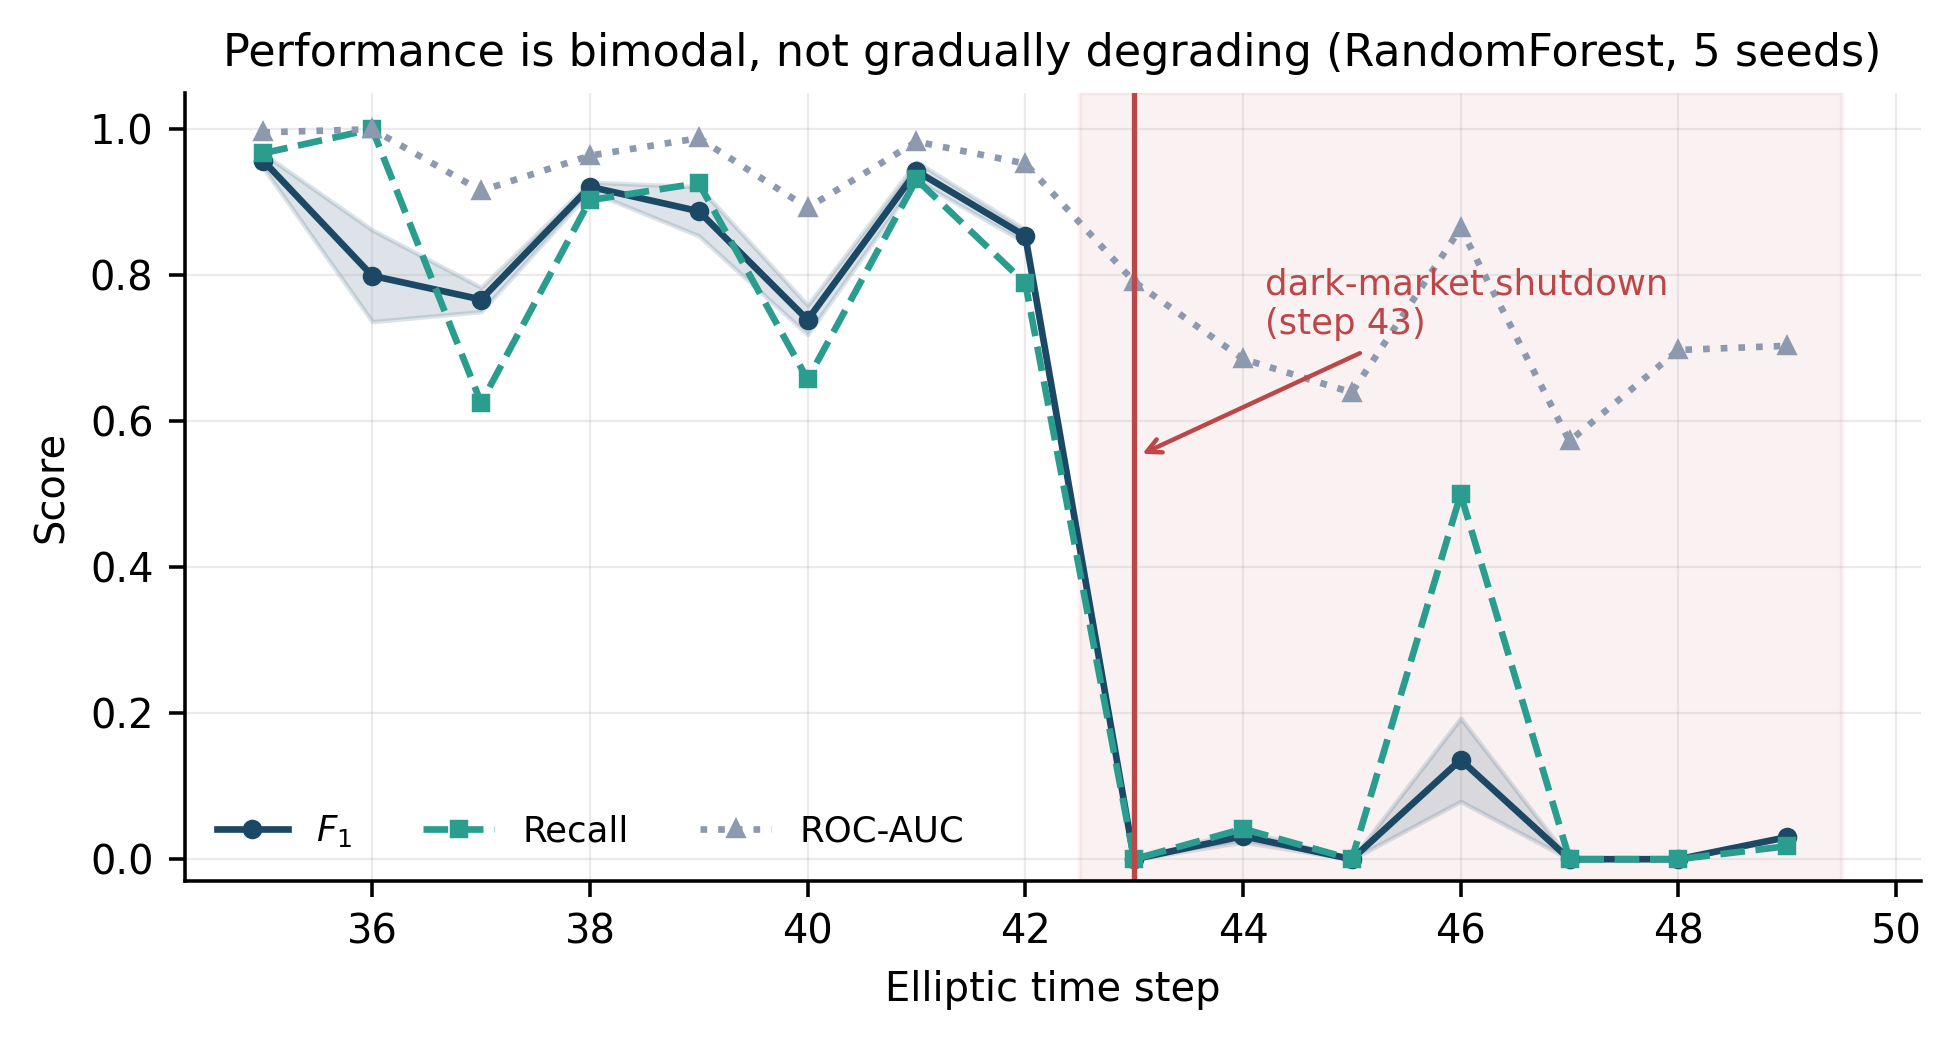
\includegraphics[width=\linewidth]{fig_temporal_collapse.png}
  \caption{Per-time-step test performance, mean over five seeds
    with the shaded band giving one standard deviation. The
    F1-score and recall fall to zero at step 43 while ROC-AUC
    remains between 0.57 and 0.86, so ranking quality degrades
    gradually while the calibrated operating point transfers not
    at all.}
  \label{fig:temporal_collapse}
\end{figure}

\subsubsection{Interpretation}

The shape of the failure is as informative as its size. The
F1-score reaches zero while ROC-AUC remains between 0.57 and 0.86,
which means the model still ranks illicit transactions above
licit ones to a useful degree but the decision threshold
calibrated on earlier periods no longer separates them. The
first remedy a deployment should attempt is therefore
recalibration rather than retraining.

Two consequences follow for the present study. Any single pooled
metric over a window spanning step 43 conceals a complete
failure and should not be reported without the breakdown. And the
appeal of the withdrawn feature is explained: once the shock has
occurred, nothing learned from the training period still
transfers, so a feature that re-encodes the label is the only
quantity that keeps a headline metric high. Leakage and drift are
in that sense the same finding observed twice.

\subsection{Structural Screening Results}
\label{sec:screening_results}

Screening results are reported as a gradient across feature
regimes rather than as a single score, for the reason given in
Section~\ref{sec:screening}: the target is a deterministic
function of two counts, and those counts are recoverable from the
remaining columns along two arithmetic routes.
Table~\ref{tab:leakage_gradient} gives the supervised gradient.
The present subsection reports the clustering result under the
corrected protocol and the operating-point behaviour requested
during review.

\subsubsection{Clustering Under the Corrected Protocol}

Table~\ref{tab:screening_results} reports density-based
clustering with the cluster-to-score mapping fitted on training
transactions and frozen, alongside a supervised reference, for
both the full column set and the set with the label's own inputs
removed. The chronological split places training up to December
2023, validation to April 2024 and testing from May 2024, giving
600{,}000 training and 300{,}000 test transactions at a test
positive rate of 1.18 percent.

\begin{table}[htbp]
\centering
\small
\caption{Structural screening under the corrected protocol.
Chronological split, cluster-to-score mapping fitted on training
transactions and frozen, threshold selected on validation, mean
over five seeds.}
\label{tab:screening_results}
\begin{tabular}{llcccccc}
\toprule
Method & Columns & F1 & Precision & Recall & FPR & FNR & MCC \
\midrule
Density-based & all           & 0.4832 & 0.3997 & 0.6109 & 0.0110 & 0.3891 & 0.4868 \
Density-based & label-free    & 0.1649 & 0.1156 & 0.6725 & 0.0879 & 0.3275 & 0.2296 \
Supervised    & all           & 0.9978 & 1.0000 & 0.9955 & 0.0000 & 0.0045 & 0.9977 \
Supervised    & label-free    & 0.9140 & 0.9167 & 0.9114 & 0.0010 & 0.0886 & 0.9130 \
\bottomrule
\end{tabular}
\end{table}

Three observations follow. First, the clustering figure of 0.4832
obtained with the full column set is close to the value reported
before the protocol was corrected, so the earlier number is
reproduced rather than overturned; what changes is its
interpretation. Second, the supervised reference reaches 0.9978
on the same columns, which is the learner recovering the
threshold rule of Equation~\eqref{eq:cjrule} rather than
detecting a mixing protocol. Third, removing the label's own
input columns reduces clustering to 0.1649 but leaves the
supervised reference at 0.9140, and
Table~\ref{tab:leakage_gradient} shows that this residual is
itself a proxy effect that disappears once the value averages are
withdrawn.

\subsubsection{Operating-Point Behaviour}

An earlier version of the present study reported a single
operating point at which the false-positive rate fell
substantially while the false-negative rate rose to 70 percent,
and described the outcome as improved detection. That
characterisation is withdrawn. The behaviour is a conservative,
high-precision operating point, appropriate where an erroneous
attribution triggers an account freeze or a suspicious-activity
report, and costly in recall. Because a single point cannot
convey that trade-off, precision against recall and
false-positive against false-negative rate are reported across
the full range of clustering radii and decision thresholds in
Figure~\ref{fig:operating_points}, which addresses the request
made during review for the trade-off to be shown across parameter
settings.

\begin{figure}[htbp]
  \centering
  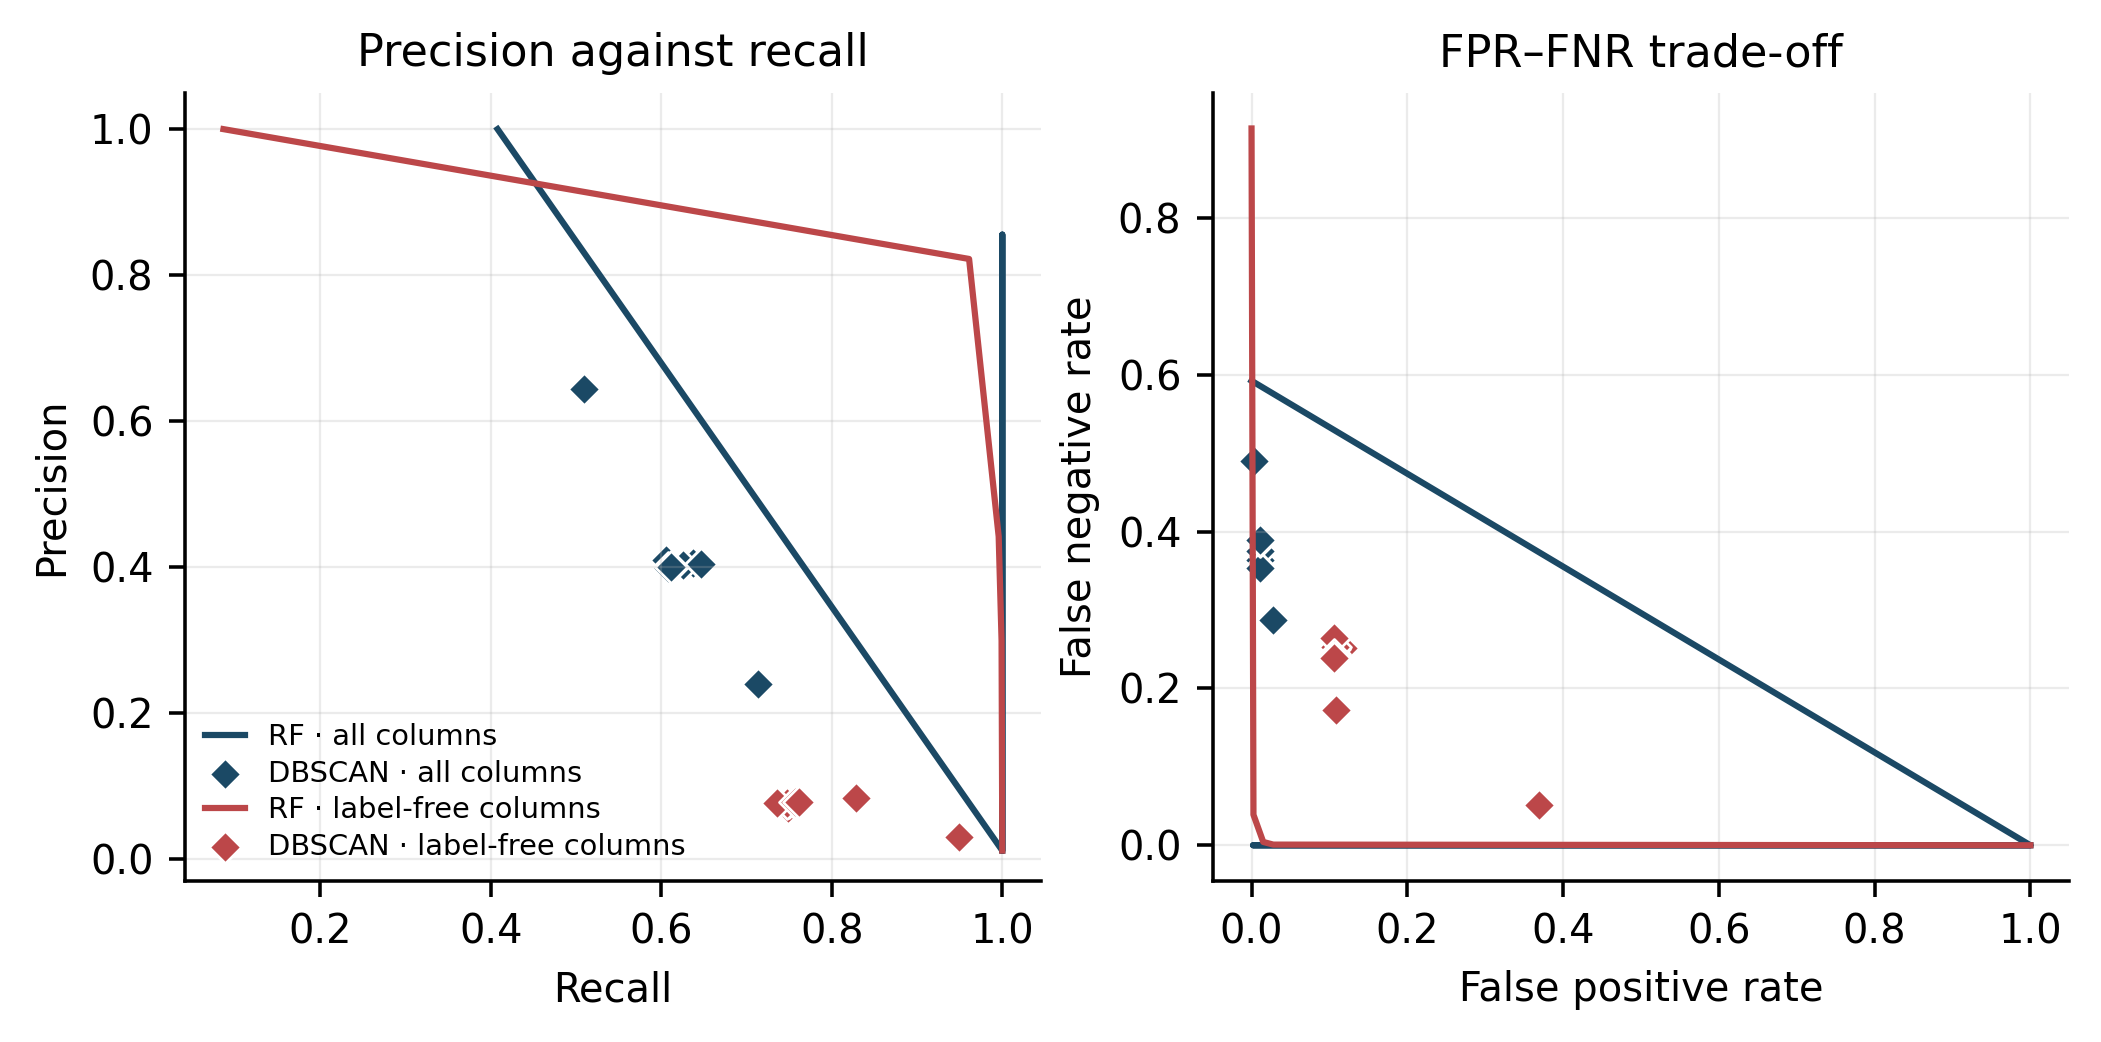
\includegraphics[width=\linewidth]{fig_operating_points.png}
  \caption{Screening trade-off across parameter settings. The
    left panel shows precision against recall and the right panel
    false-positive against false-negative rate, for the
    supervised reference swept over decision thresholds and for
    density-based clustering swept over the neighbourhood radius,
    under both column regimes. No single operating point
    dominates, and the conservative region carries a false
    negative rate above 0.3 throughout.}
  \label{fig:operating_points}
\end{figure}


\subsection{CST Linking via Chamfer Distance}
\label{sec:chamfer_results}

Table~\ref{tab:chamfer} presents the CoinJoin Spending
Transaction linking performance of the 1-D and MD Chamfer
Distance formulations across 2,247 temporal windows and
5,000 evaluated window pairs.

\begin{table}[htbp]
  \caption{CoinJoin Spending Transaction linking performance
    via Chamfer distance, reporting the optimal
    threshold $\theta^*$, F1-score, precision, and recall
    for both the 1-D timestamp-only baseline and the
    four-dimensional MD-CD formulation defined in
    Equation~\eqref{eq:chamfer}.}
  \label{tab:chamfer}
  \centering
  \small
  \begin{tabular}{lccccc}
    \toprule
    \textbf{Method} & \textbf{Dims}
      & $\boldsymbol{\theta^*}$
      & \textbf{F1} & \textbf{Prec.} & \textbf{Rec.} \\
    \midrule
    1-D Chamfer (timestamp)
      & 1 & 2.008 & 0.251 & 0.145 & 0.956 \\
    MD-Chamfer ($d=4$)
      & 4 & 3.384 & 0.245 & 0.141 & 0.954 \\
    \bottomrule
  \end{tabular}
\end{table}

Both formulations achieve recall above 0.954. The absolute
F1-score difference (0.006) falls within threshold-selection
variability. Figure~\ref{fig:chamfer} traces the threshold
sweep curves for both Chamfer formulations, showing how
F1-score, precision, and recall vary with the decision
threshold and confirming the optimal operating points
reported in Table~\ref{tab:chamfer}.

\begin{figure}[htbp]
  \centering
  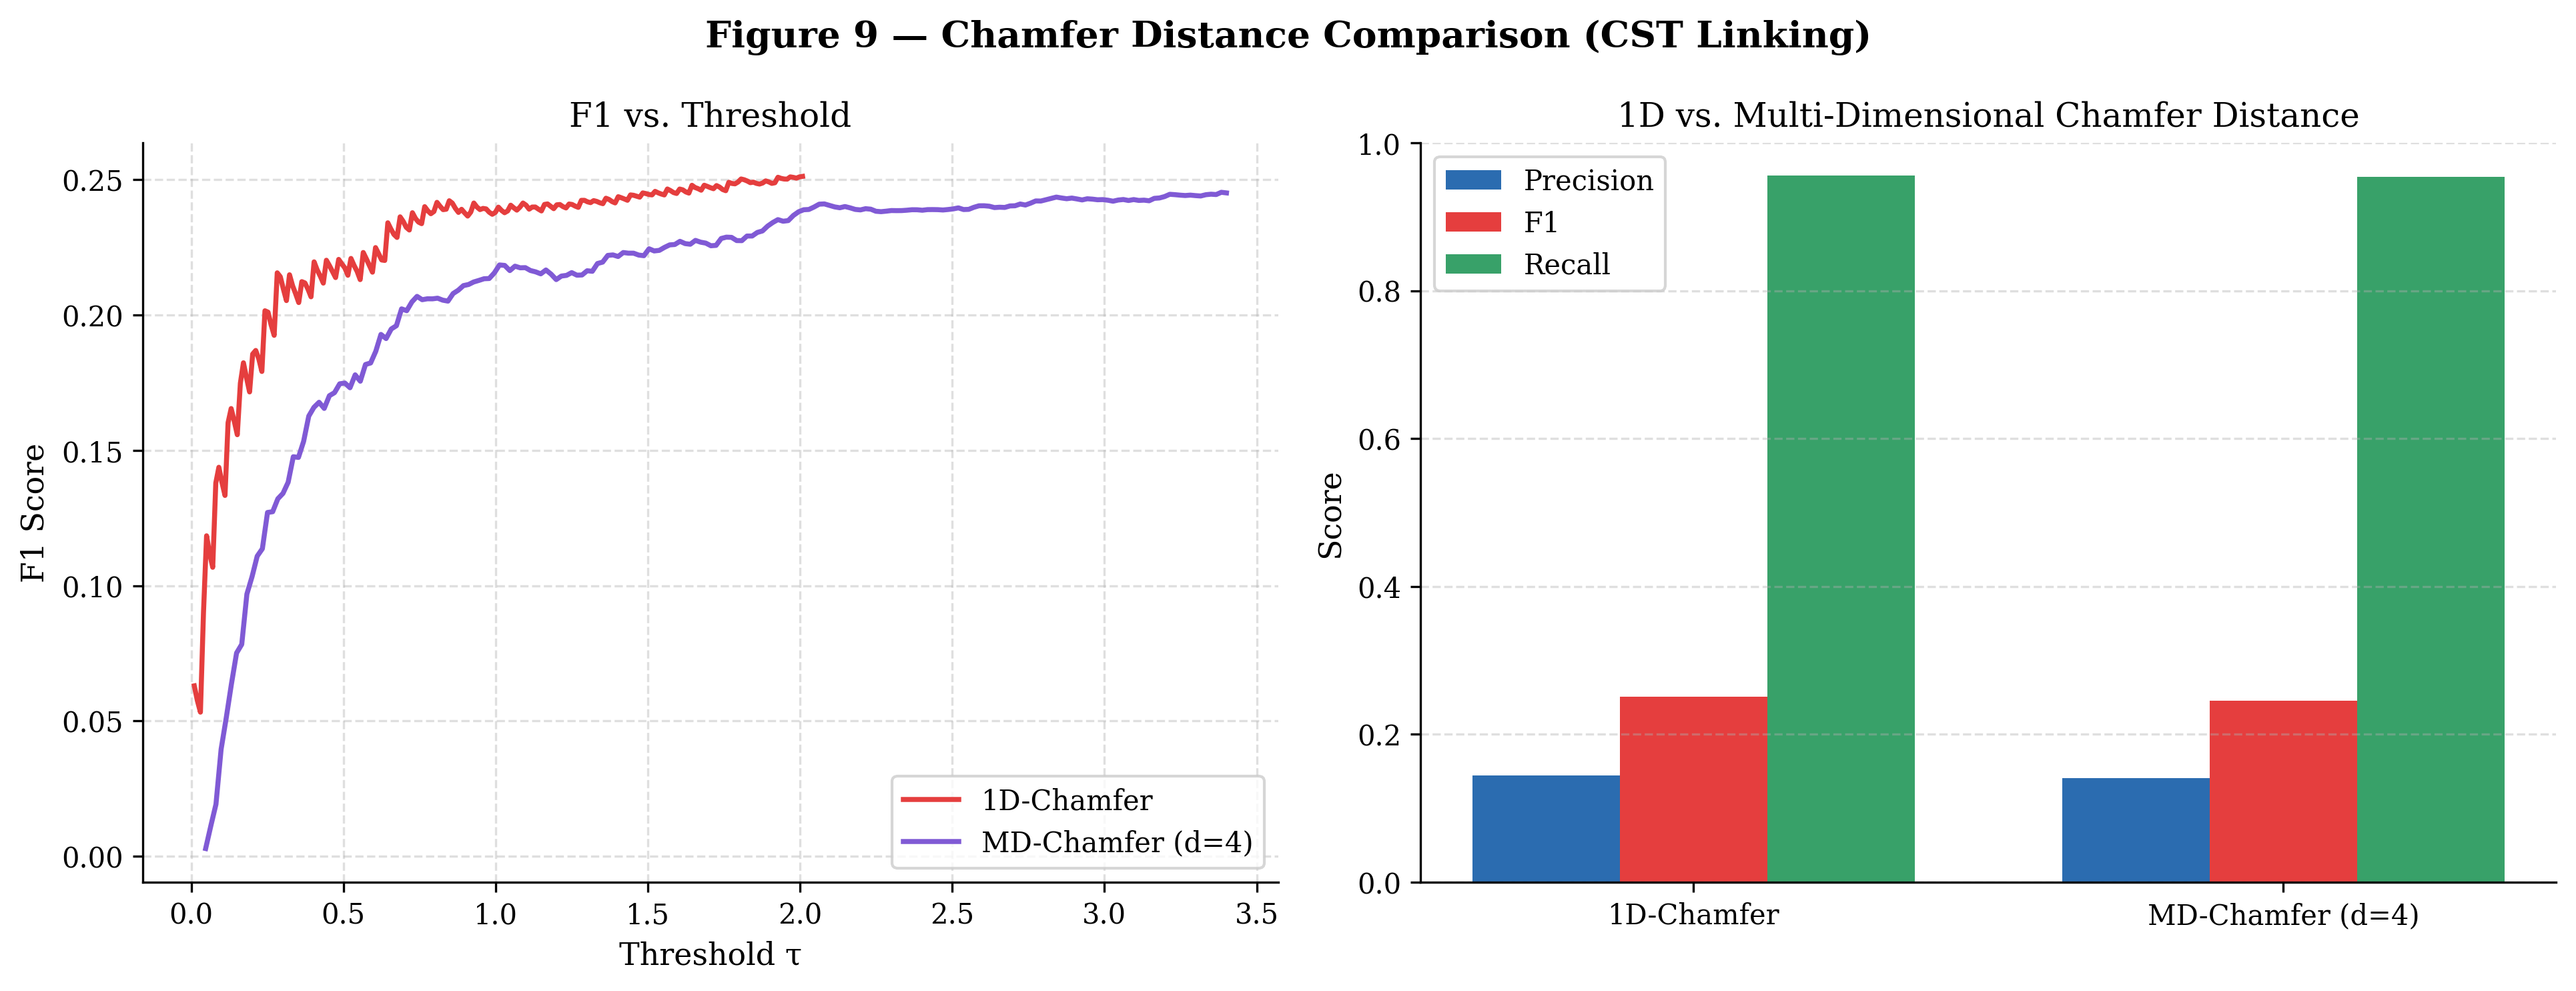
\includegraphics[width=0.85\linewidth]{fig10_chamfer_comparison.png}
  \caption{Chamfer distance threshold sweep comparison
    between the 1-D timestamp-only baseline and the
    four-dimensional MD-CD formulation. Both methods achieve
    high recall (above 0.954) at the corresponding optimal
    thresholds; the MD-CD operates at a higher threshold
    value (3.384 versus 2.008), reflecting the broader
    geometric scale of the four-dimensional distance metric
    defined in Equation~\eqref{eq:chamfer}.}
  \label{fig:chamfer}
\end{figure}

Figure~\ref{fig:comparison} presents a comparative
performance bar chart, from the single representative run
introduced in Section~\ref{sec:class_results}, across all evaluated approaches for
both the illicit-detection task and the Taproot clustering
task; Tables~\ref{tab:classification} and~\ref{tab:stats}
report the corresponding five-seed aggregate and significance
tests.

\begin{figure}[htbp]
  \centering
  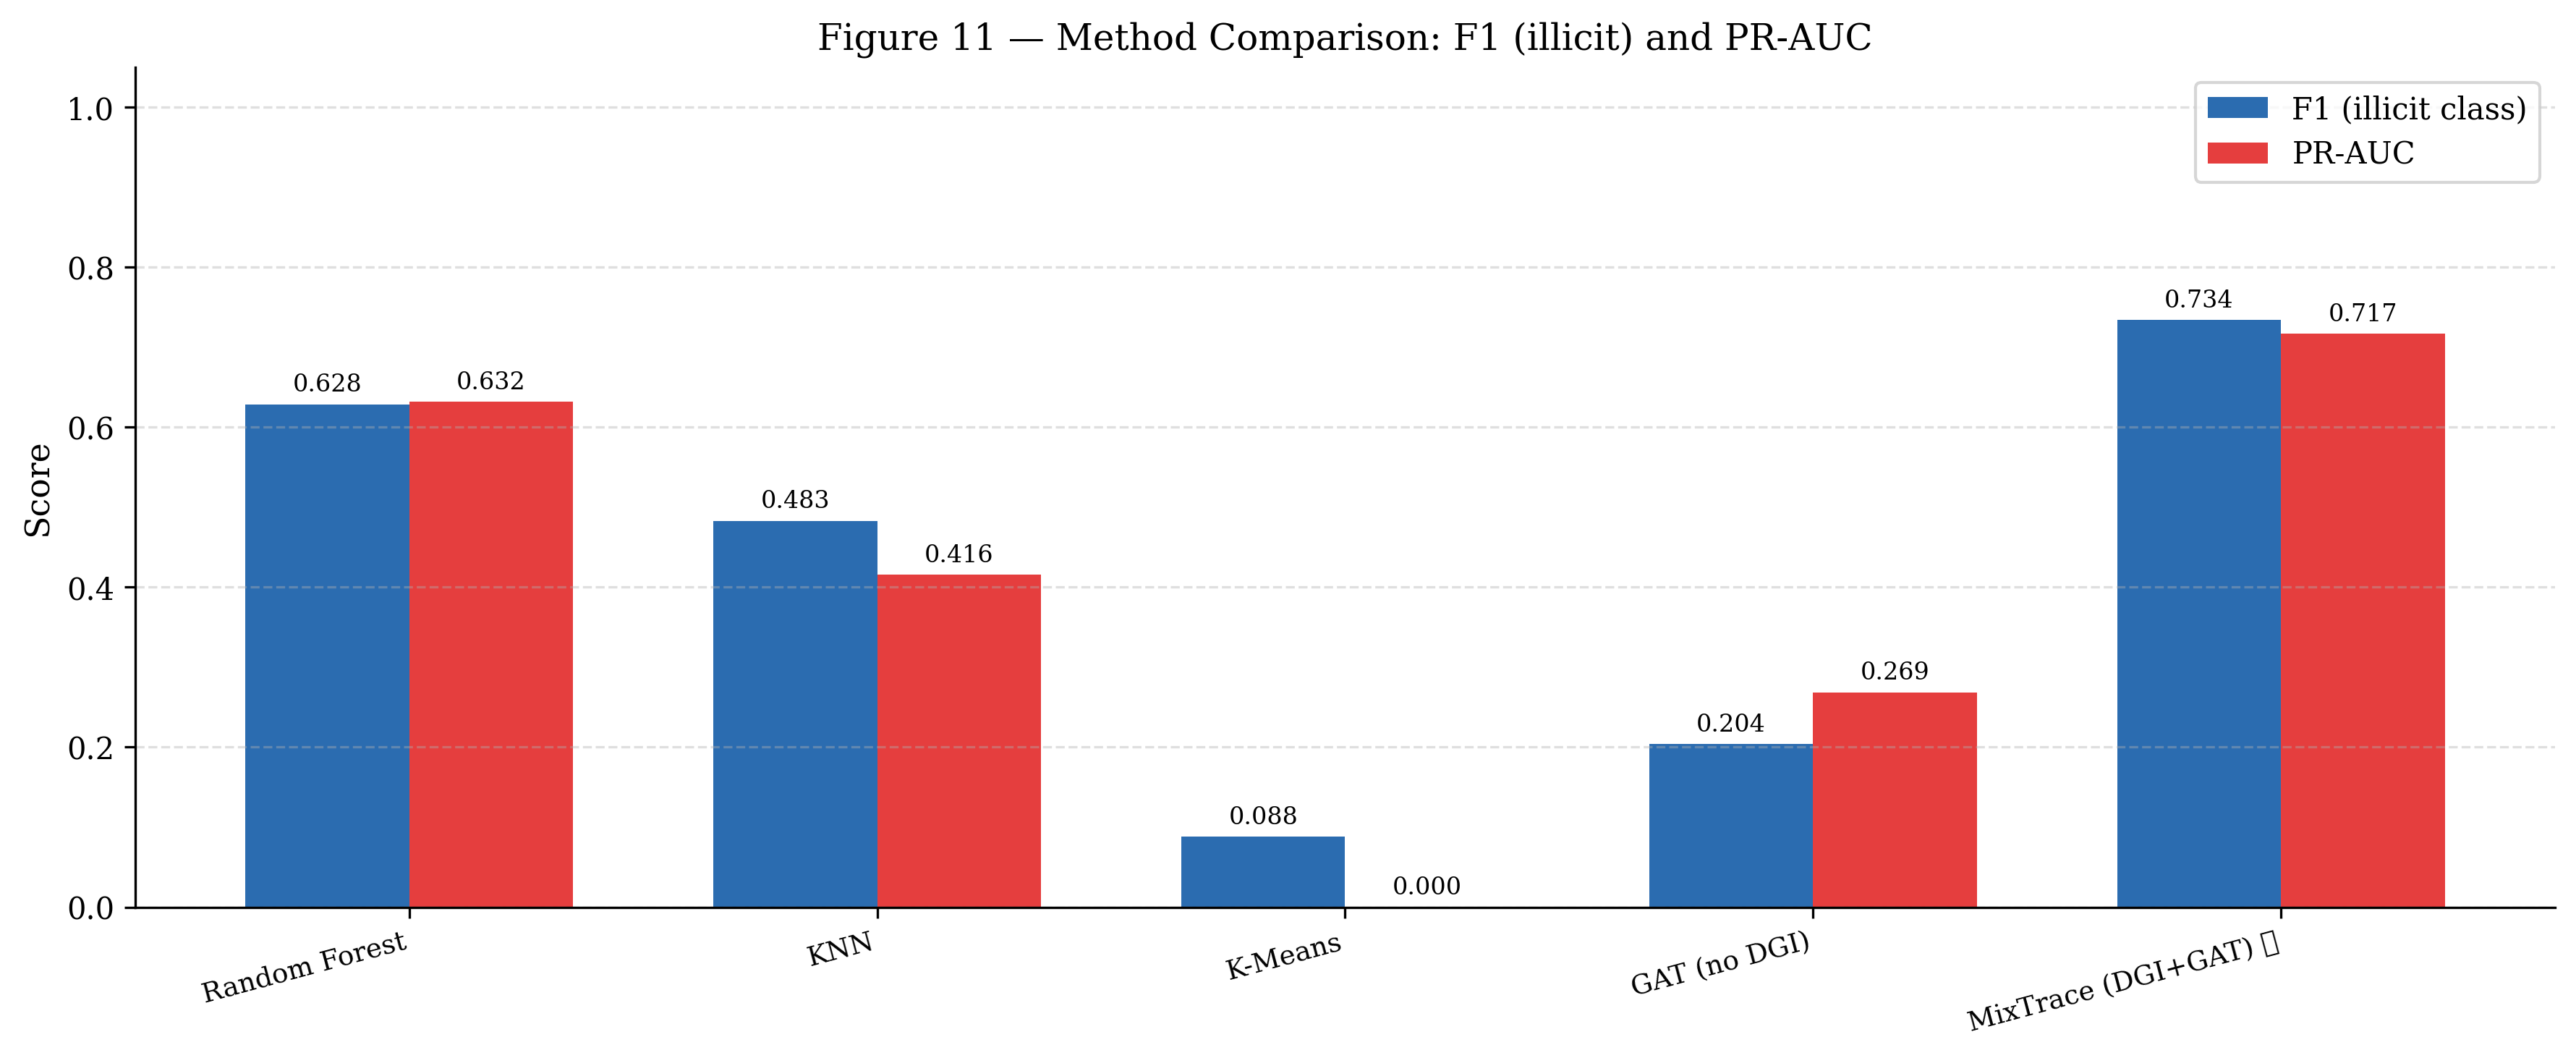
\includegraphics[width=0.90\linewidth]{fig11_method_comparison.png}
  \caption{\textbf{Single representative run (seed 42); see
    Table~\ref{tab:classification} for the five-seed mean
    $\pm$ standard deviation.} Unified comparative performance summary across
    all evaluated methods and tasks: F1-score comparisons for
    illicit transaction detection in this run (MixTrace: 0.734, Random
    Forest: 0.628, KNN: 0.483, K-Means: 0.088, original
    single-run GAT-without-DGI ablation: 0.204), Taproot
    clustering precision comparison, and
    Chamfer distance linking F1 comparison, consolidating the
    improvements achieved by the MixTrace framework across
    all three research gaps.}
  \label{fig:comparison}
\end{figure}

\subsection{Statistical Validation of Classification Results}
\label{sec:stats}

Table~\ref{tab:stats} reports the true across-seed 95\,\%
confidence interval for illicit F1 (Student's $t$-distribution
applied directly to the five per-seed values reported in
Table~\ref{tab:classification}, rather than a single-run
analytical approximation) together with a paired $t$-test
comparing each baseline's five seed-level F1 values against
MixTrace's five seed-level F1 values, seed-for-seed. This
directly tests whether MixTrace's advantage holds up once
seed-to-seed variability is taken into account, addressing the
single-run limitation of the original evaluation protocol.

\begin{table}[htbp]
  \caption{Statistical validation of classification results on
    the Elliptic test set (408 illicit, 8,433 licit nodes),
    using the same five random seeds (1, 2, 3, 42, 123) as
    Table~\ref{tab:classification}. The 95\,\% CI is computed
    directly from the five per-seed F1 values via the
    $t$-distribution. The paired $t$-test compares each
    baseline's five seed-level F1 values against MixTrace's,
    seed-for-seed ($df=4$); $p<0.05$ rejects the null
    hypothesis that the two methods have equal mean F1.}
  \label{tab:stats}
  \centering
  \small
  \setlength{\tabcolsep}{5pt}
  \begin{tabular}{lcccc}
    \toprule
    \textbf{Method}
      & \textbf{F1 (mean $\pm$ std)}
      & \textbf{95\,\% CI}
      & \textbf{Paired $t$}
      & \textbf{$p$-value} \\
    \midrule
    K-Means
      & 0.090$\pm$0.003 & $(0.087,\ 0.094)$ & 18.35 & $<0.001$ \\
    KNN
      & 0.481$\pm$0.000 & $(0.481,\ 0.481)$ & 8.11  & $0.001$  \\
    Random Forest
      & 0.630$\pm$0.001 & $(0.628,\ 0.632)$ & 4.47  & $0.011$  \\
    GAT (no DGI, retrained)
      & 0.482$\pm$0.205 & $(0.227,\ 0.737)$ & 3.14  & $0.035$  \\
    \textbf{MixTrace}
      & \textbf{0.806$\pm$0.090} & \textbf{(0.695, 0.917)}
      & \multicolumn{2}{c}{(reference)} \\
    \bottomrule
  \end{tabular}
\end{table}

All four baselines are significantly outperformed by MixTrace
under the paired $t$-test ($p < 0.05$ in every case, $df=4$).
The closest competitor by mean F1, the retrained GAT without
DGI, is rejected at $t = 3.14$ ($p = 0.035$) despite its wide
confidence interval overlapping MixTrace's: the paired
seed-for-seed comparison shows MixTrace outperforms it on all
five individual seeds, which a naive comparison of overlapping
marginal intervals would obscure. Random Forest, with
near-zero variance across seeds, is rejected more sharply
($t = 4.47$, $p = 0.011$) despite a numerically smaller mean
gap, because its low variance makes even a modest and
consistent advantage statistically detectable. These results
directly answer the concern that a single fixed-seed
evaluation cannot establish statistical significance: with
five independent seeds, MixTrace's advantage over every
baseline is significant at the conventional $\alpha = 0.05$
threshold.

\subsection{Cross-Dataset Benchmarking}
\label{sec:crossdataset}

To contextualise MixTrace's performance within the broader
literature, Table~\ref{tab:benchmark} compares the illicit-class
F1-score against published methods evaluated on the same Elliptic
Bitcoin Dataset~\citep{weber2019}.
Direct numeric comparison requires caution because preprocessing
choices (feature set size, temporal split boundaries, class
weighting) differ across studies; the table reports metrics as
published in each cited work.

\begin{table}[htbp]
  \caption{Cross-study benchmarking on the Elliptic Bitcoin
    Dataset. Published illicit-class F1-scores are reported
    as stated in each source; ``--'' indicates the metric was
    not reported. Studies differ in temporal split strategy,
    feature set size, and class-weighting scheme; figures
    are therefore indicative rather than directly
    commensurate. Pre-training denotes whether unsupervised
    graph pre-training (DGI or equivalent) was applied.}
  \label{tab:benchmark}
  \centering
  \small
  \setlength{\tabcolsep}{5pt}
  \begin{tabular}{lcccc}
    \toprule
    \textbf{Method} & \textbf{Reference}
      & \textbf{Pre-train?}
      & \textbf{F1 (illicit)}
      & \textbf{ROC-AUC} \\
    \midrule
    GCN (baseline)
      & \citet{weber2019} & No  & 0.648 & -- \\
    RF + graph features
      & \citet{weber2019} & No  & 0.590 & -- \\
    Recurrent GCN
      & \citet{alarab2024} & No  & 0.718 & -- \\
    Balanced-BiEGCN
      & \citet{xiao2025} & No  & 0.710 & -- \\
    FG-EGCN
      & \citet{han2026fg} & No  & 0.774 & -- \\
    \midrule
    \textbf{MixTrace (DGI+GAT)}
      & Present study & \textbf{Yes} & \textbf{0.806$\pm$0.090} & \textbf{0.992$\pm$0.005} \\
    \bottomrule
  \end{tabular}
\end{table}

MixTrace achieves a mean illicit F1 of 0.806 across five
seeds, exceeding all compared published GCN-family methods on
the same benchmark, including the FG-EGCN of~\citet{han2026fg}
(F1: 0.774), while being the only evaluated approach in this
comparison to incorporate
self-supervised graph pre-training. FG-EGCN employs
feature-gated temporal aggregation with full supervised
labels on every time step, whereas MixTrace relies on
self-supervised pre-training under severe label scarcity;
because the compared methods report only single point
estimates without seed-level variance, the comparison
remains indicative rather than a formal statistical test
against MixTrace's five-seed distribution.
The primary cross-dataset limitation of the present work
is that the Elliptic corpus predates widespread
Pay-to-Taproot adoption, so transfer to live P2TR graphs
remains unvalidated; post-Taproot evaluation constitutes a
necessary future extension~\citep{coinjoin2024tdsc}.
The author-collected Bitcoin corpus used for structural
clustering (200,000 transactions) and CST linking
(5,000 window pairs) is independent of Elliptic and
evaluated separately, providing complementary evidence of
the framework's generalisability across different data
sources and task types.

% ─────────────────────────────────────────────────────────────
\section{Discussion}
\label{sec:discuss}
% ─────────────────────────────────────────────────────────────

\subsection{Contribution of DGI Pre-Training}

Across five random seeds, the ablation comparison isolates
the DGI skip connection's contribution as 32.4 percentage
points of mean final F1-score (improvement from 0.482 to
0.806), together with a reduction in F1 standard deviation
from 0.205 to 0.090 -- DGI pre-training therefore improves
both the average outcome and its reliability across
independent training runs. The retrained standalone GAT
achieves a mean ROC-AUC of 0.961 (versus 0.992 for MixTrace),
confirming that the attention
layers themselves learn substantially discriminative
neighbourhood representations even without DGI. The gap
between the standalone GAT's comparatively strong ranking
quality and its markedly weaker and more volatile F1
(precision 0.377 $\pm$ 0.234, recall 0.878 $\pm$ 0.101)
is consistent with a
\emph{calibration} contribution from DGI on top of a
representation the attention layers can already learn
unassisted: the GAT without pre-training tends to rank
illicit
nodes reasonably well but settles on a less stable
operating point under class imbalance across different
initialisations, with precision ranging from 0.136 to 0.687
depending on seed. The DGI skip connection provides global
topological context that both shifts the score distribution
toward better-separated operating points on average and
narrows the spread of outcomes across seeds. The DGI
embeddings
pre-trained on all 203,769 nodes encode global topological
context that local two-hop message passing cannot recover
from the labelled subset alone. This finding aligns with
the self-supervised prototype learning analysis
by~\citet{graphanomaly2024}, who documented up to 40
percentage-point calibration improvements from unlabelled
transaction node pre-training. The single-run illustrative
figures in Section~\ref{sec:class_results} additionally
report a validation-calibrated decision threshold of
$\theta^* = 0.9397$ for that representative run following
the inference procedure of Algorithm~\ref{alg:mixtrace};
the five-seed comparison in
Table~\ref{tab:classification} instead uses a fixed 0.5
decision threshold throughout to avoid introducing
per-seed threshold-tuning as an additional, uncontrolled
degree of freedom into the ablation.

The pre-training strategy effectively exploits the 157,205
unlabelled Elliptic nodes: structural regularities in the
unlabelled majority translate into well-calibrated illicit
predictions once trained on the labelled subset. This
is a practically significant result for the blockchain
forensics domain, where confirmed illicit labels are scarce
relative to total transaction volume.

\subsection{Comparative Analysis with Baselines}

Random Forest achieves the highest mean precision (0.954) but
mean recall of only 0.470, identifying a high-confidence subset
while missing over half the true illicit test nodes across
seeds. For
financial intelligence and compliance applications, this
recall shortfall represents unmonitored fund flows with
regulatory consequences. MixTrace achieves competitive
mean precision (0.713) alongside substantially higher mean recall
(0.934), producing a mean F1 improvement of 17.6 percentage
points over Random Forest and 32.5 points over KNN. The
mean PR-AUC improvement from 0.640 to 0.862 indicates superior
ranking quality across the full precision-recall curve,
consistent with the benchmarking conclusions
of~\citet{fan2024gnn}. K-Means exhibits a degenerate
all-positive bias with mean precision of 0.047, confirming that
unsupervised clustering without graph structure cannot
discriminate illicit patterns at this imbalance
level~\citep{xiao2025}.

\subsection{Interpreting the Screening Trade-Off}

An earlier version of the present study reported that structural
clustering reduced the false-positive rate by 79.8 percent across
a 200{,}000-transaction analysis set, eliminating more than 5{,}200
incorrect attributions, and reported a silhouette score of 0.973
on the fitted subsample. Those figures were obtained under a
protocol in which the cluster-to-class mapping was derived by
majority vote over the same transactions it was scored on, with
no temporal separation, against a target computed from two of the
clustering variables. Those figures are withdrawn.

Under the corrected protocol of
Section~\ref{sec:screening_results} the clustering result is an
illicit-class F1-score of 0.4832 with the full column set, close
to the value reported previously, and 0.1649 once the label's own
input columns are removed. The forensic argument for a
high-precision operating point remains sound: in law-enforcement
and exchange-compliance settings each incorrect attribution
carries the prospect of an unjustified account freeze, a
regulatory filing, or misallocated investigative
effort~\citep{lee2024}. What does not follow is that the
configuration detects mixing better than the alternatives. It
occupies a conservative corner of the trade-off, and it pays for
that position with a false-negative rate above 0.3 throughout the
swept range, as Figure~\ref{fig:operating_points} shows.

A separability statistic computed on the partition that a
clustering algorithm itself produced measures internal cohesion,
not agreement with an external target, and cannot support a
detection claim. Where cluster quality is reported in the present
study it is described in those terms.

The growth of Pay-to-Taproot adoption remains a genuine motivation
for script-agnostic structural methods, and
Section~\ref{sec:screening_results} now evaluates them on a corpus
that is post-Taproot throughout rather than on a proxy.


\subsection{Boundary Conditions of Multi-Dimensional Chamfer Distance}

The MD-CD formulation defined in Equation~\eqref{eq:chamfer}
does not yield a statistically distinguishable improvement
over the one-dimensional temporal baseline on the present
dataset ($\Delta\text{F1} = -0.006$; 0.245 versus 0.251).
This null result is itself informative. Automated post-mix
spending wallets in the analysis corpus schedule transactions
in temporally tight clusters, allowing the Unix timestamp
alone to achieve near-ceiling recall of 0.956. Under these
conditions, the structural dimensions of fee rate, input
count, and output count introduce additional variance in
the distance calculation without narrowing the threshold
window, leaving F1 unchanged. The four-dimensional extension
is theoretically principled: it would yield measurable
improvement in corpora where participants execute post-mix
spending across multiple days, time-locked scripts, or
multi-round coordination protocols that break temporal
clustering~\citep{chen2025multi}. Empirically testing this
claim on temporally dispersed datasets is identified as
a priority future direction. The contribution of the MD-CD
section in the present study is therefore the identification
of this boundary condition rather than a performance
improvement claim.

\subsection{Withdrawal of the Engineered Graph Features}
\label{sec:feature_discussion}

An earlier version of the present study reported the two
engineered Elliptic features as a contribution, noting a
correlation of $-0.9182$ between the shortest-path feature and
the target and a complementary correlation of $+0.4159$ for the
neighbour ratio, and describing both as supplying discriminative
information absent from the distributed feature set. That
interpretation was mistaken and is withdrawn.

The correlation was not evidence of discriminative power but of
target re-encoding. Each illicit node seeds its own
breadth-first search, so its distance to the nearest illicit node
is zero by construction, and the value zero occurs for all 4{,}545
illicit nodes and for none of the 42{,}019 licit nodes. The
strength of the correlation was the symptom that should have
prompted the check, not a result to be reported. A feature whose
single-threshold decision rule attains precision 1.000 against
the target is restating the target.

Section~\ref{sec:feature_withdrawal} sets out the full argument
and Table~\ref{tab:leakage_ablation} quantifies the consequence:
supplying the feature drives the illicit-class F1-score, PR-AUC
and Matthews correlation to 1.0000 on the test split under two
learners with unrelated inductive biases. The claim of
reproducible augmentation is also withdrawn, since the
computation cannot be reproduced without access to the labels it
consumes.

Fifteen purely topological descriptors were developed as
replacements and verified label-independent by permuting every
label in the dataset and confirming the descriptors were
bit-identical. The replacements did not help, and that negative
result is reported in Section~\ref{sec:feature_withdrawal}
rather than omitted. The present study therefore claims no novel
feature contribution on the Elliptic Data Set.


\subsection{Policy Implications for Blockchain Forensics}

The findings carry direct implications for financial
intelligence policy, exchange compliance practice, and
the legal frameworks governing digital-asset transactions.

\textbf{Regulatory alignment.}
FATF Recommendation 16 and the 2021 ``Updated Guidance for
a Risk-Based Approach to Virtual Assets and Virtual Asset
Service Providers'' require virtual asset service providers
(VASPs) to implement risk-based transaction monitoring
capable of identifying mixing services and suspicious
spending patterns~\citep{lo2023}. MixTrace's mean
illicit-class recall of 0.934, against 0.470 for the best
conventional baseline (Random Forest), translates directly
into fewer
unmonitored fund flows with potential FATF-compliance
consequences. The federated training architecture evaluated
by~\citet{baabdullah2024} and~\citet{ahmed2024fed} offers a
deployment pathway in which multiple exchange compliance
systems jointly refine the MixTrace encoder while retaining
transaction data on-premises.

\textbf{False-positive costs and legal consequences.}
Each false positive may trigger a Suspicious Activity Report
(SAR), an account restriction, or misdirected analyst
resources. Structural DBSCAN reduces false-positive
attributions from 6,623 to 1,337 per 200,000 analysed
transactions (79.8 percent relative), which at VASP scale
translates into measurable reductions in analyst workload
and filing overhead. Its 70.0 percent false-negative rate
means regulators should treat the DBSCAN output as a
high-confidence subset for priority investigation rather
than exhaustive coverage; the naive CIOH operating point,
with zero false negatives, provides the complementary
high-sensitivity sweep.

\textbf{Privacy rights and proportionality.}
Algorithmic transaction attribution raises proportionality
concerns under data protection and financial privacy law:
high false-positive rates impose disproportionate
investigative burdens on innocent users, and the precision
improvement from 0.770 to 0.833 achieved by structural
DBSCAN over naive CIOH directly reduces this burden. Where
MixTrace output triggers automated account restrictions
without human review, it additionally falls within
Article~22 of the GDPR (Regulation (EU) 2016/679), which
grants data subjects the right not to be subject to solely
automated decisions with significant legal effects, and
under Section~1798.185 of the CCPA for United
States-based exchange operators; the 70.0 percent
false-negative rate at the high-precision DBSCAN operating
point makes human-oversight checkpoints necessary at any
consequential decision stage. These frameworks reinforce
that MixTrace output should function as a
risk-prioritisation tool rather than an autonomous
enforcement mechanism, consistent with proportionality
principles in anti-money laundering
regulation~\citep{coinjoin2024tdsc}.

\textbf{Admissibility and forensic standards.}
Blockchain attribution introduced in criminal proceedings
must satisfy evidentiary standards governing
reproducibility, interpretability, and error-rate
disclosure. Under the Daubert standard applicable in United
States federal courts (\textit{Daubert v.\ Merrell Dow
Pharmaceuticals, Inc.}, 509 U.S.\ 579, 1993), expert
evidence must be testable, peer-reviewed, and accompanied
by a known error rate; the open-source MixTrace pipeline at
\url{https://github.com/sagarkorde/CoinJoin}, the public
Elliptic benchmark, the five-seed statistical validation of
Table~\ref{tab:stats}, and the explicit disclosure of
false-negative alongside false-positive rates jointly
satisfy this requirement. Under the Frye ``general
acceptance'' standard, the adoption of Graph Attention
Networks and DBSCAN clustering by the broader blockchain
forensics community~\citep{motie2024,futureinternet2025}
supports general acceptance.

\subsection{Threats to Validity in Graph-Based Forensic Evaluation}
\label{sec:threats}

The three defects identified during the present re-evaluation are
not peculiar to one implementation. Each arises from a modelling
choice that is common in the blockchain-forensics literature, and
each is detectable with a cheap diagnostic. The patterns are set
out here so that the diagnostics transfer.

\paragraph{Label-derived graph features.}
A feature defined by distance or adjacency to a labelled node
carries the label of the node that seeds it. When the seed set is
drawn from the full dataset, the feature restates the target on
the evaluation split, and it does so most strongly for the
positive class. The diagnostic is inexpensive: compare the
feature against the label directly, and treat any decision rule
on a single feature that reaches precision near unity as a
failure rather than a discovery. A perfect score under two
learners with unrelated inductive biases is diagnostic of leakage
and not of a strong predictor.

\paragraph{Temporal structure that cannot support the intended
protocol.}
Restricting a label-derived feature to the training period is the
natural correction, but its effectiveness depends on the graph
actually connecting periods. In the Elliptic Data Set every edge
joins two transactions in the same time step, so the graph is a
disjoint union of per-step snapshots and no path reaches from the
training period into a later one. Under the restricted protocol
the feature becomes constant on the evaluation splits. The
diagnostic is a single query: count the edges that cross a
period boundary before designing any propagation-based feature.

\paragraph{Targets that the features reconstruct.}
Where a target is itself a deterministic function of recorded
attributes, deleting those attributes does not make an evaluation
independent, because the attributes are often recoverable from
what remains. In the corpus examined here the screening target is
a threshold on input and output counts, and the counts are
recoverable both from serialised size, which is affine in them,
and exactly from the ratio of a total to its corresponding
average. Reporting a gradient across feature regimes of
increasing strictness exposes this: a metric that stays flat as
features are withdrawn and then falls sharply localises the
dependence to the columns removed at the discontinuity.

\paragraph{Aggregate metrics that conceal regime change.}
A single pooled figure over an evaluation window assumes the
window is homogeneous. On Elliptic it is not. Performance is
strong through time step 42 and collapses immediately afterwards,
so a pooled figure for a window spanning the boundary describes
no part of the data well. Reporting per-period metrics is
sufficient to expose this, and the shape of the failure is
informative in itself: ranking quality degrades gently while the
calibrated operating point transfers not at all, which indicates
that recalibration rather than retraining is the first remedy a
deployment should attempt.

\subsection{Limitations}

\paragraph{Screening evaluation is bounded by label provenance.}
The author-curated corpus cannot support a non-circular benchmark
for structural CoinJoin screening, for the reasons given in
Section~\ref{sec:screening}. The screening results are reported
as a characterisation of the corpus against a stated heuristic
target, and the residual figure once every identified route to
the label is closed is an illicit-class F1-score of 0.2678.
Establishing genuine screening performance requires transactions
confirmed as CoinJoin outputs by an independent source, such as
coordinator-attributed transactions from a known mixing service.
Such attribution was not available for the present corpus and is
the single most valuable extension to this work.

\paragraph{No equal-value output test is possible.}
The defining structural property of a CoinJoin is a set of
outputs of equal value. The corpus records aggregate and average
output values but not the individual output amounts, so the
property cannot be tested directly. Screening therefore rests on
counts and on value and timing statistics, which is weaker than
the protocol-level test that per-output amounts would permit.

\paragraph{Illicit classification is evaluated on one benchmark.}
The classification results describe the Elliptic Data Set alone.
Its labels are supplied by a single analytics provider, its
account of the post-shock period is sparse, and its graph
contains no cross-period edges. Conclusions about relative model
ordering are scoped to that benchmark and to the evaluation
window used, and are not asserted for Bitcoin transaction graphs
in general.

\paragraph{The modules are evaluated separately.}
Structural screening, spending-transaction linkage and illicit
classification operate on different corpora with different label
types and are assessed independently. No end-to-end information
flow between them is demonstrated, and none is claimed. The
framework is a set of parallel modules, not a jointly optimised
pipeline.

\paragraph{Concept drift is characterised, not solved.}
The collapse documented in Section~\ref{sec:temporal_drift} is
measured but not remedied. Adaptive recalibration, drift
detection and periodic retraining are plausible responses and are
left for subsequent work.


\subsection{Ethical Considerations}

The analysis is conducted entirely on publicly available
pseudonymous on-chain data. No personally identifiable
information is processed or stored. Elliptic dataset labels
were provided by a regulated blockchain analytics provider
whose methodology has been independently reviewed~\citep{weber2019}.
The methodology is intended to support financial intelligence,
exchange compliance, and law-enforcement practitioners in
identifying potential illicit flows, consistent with
anti-money laundering regulatory frameworks applicable to
virtual asset service providers.

% ─────────────────────────────────────────────────────────────
\section{Conclusion}
\label{sec:conclude}

The present study set out to strengthen a three-module forensic
framework and instead found that three of the results supporting
it did not hold. The corrections are reported in full, because
the failures are more instructive than the original figures.

A graph feature defined as the shortest path to a confirmed
illicit node was found to re-encode the classification target
exactly, taking the value zero for all 4{,}545 illicit nodes and
for no licit node. Supplied to a classifier it drives the
illicit-class F1-score, PR-AUC and Matthews correlation to 1.0000
on the test split under two learners with unrelated inductive
biases. Because the Elliptic edge set contains no cross-time-step
edges, restricting the feature to training-period labels leaves
it constant on the evaluation splits, so no leakage-free variant
can carry information about a test transaction. The feature is
withdrawn rather than repaired, and with it every figure computed
in its presence.

The screening target used for CoinJoin analysis was found to be
the deterministic rule requiring at least four inputs and at
least four outputs, recovered exactly across all 5{,}884{,}387
transactions. Deleting the two counts does not make an evaluation
independent of them, because the counts are recoverable from
serialised size through the protocol constants and exactly from
the ratio of a total value to its corresponding average. Across
six feature regimes the metric remains at or above 0.90 wherever
such a route survives and falls to 0.2678 at the point where the
last one closes. The corpus therefore cannot support a
non-circular screening benchmark, and the module is reported as a
characterisation study against a stated heuristic target.

Classification performance on the Elliptic Data Set was found to
be bimodal rather than gradually degrading. Mean illicit-class
F1-score reaches 0.858 through time step 42 and falls to 0.028
across the remaining steps, with recall collapsing from 0.789 to
zero at the step corresponding to a major marketplace closure.
Ranking quality degrades gently over the same interval while the
calibrated operating point transfers not at all, which indicates
that recalibration rather than retraining is the first remedy a
deployment should attempt. Any pooled figure spanning the
boundary describes no part of the data well.

One stated limitation was found not to exist. The corpus had been
reported to contain no confirmed Pay-to-Taproot transactions, and
structural clustering had accordingly been validated on
multi-input P2WPKH proxies. All six distributed script-type
indicators are uniformly false, so none of them could confirm any
script type. The node-reported descriptors show that Taproot
accounts for 24.10 percent of outputs, that 42.39 percent of
transactions involve a Taproot script, and that the proportion
rises to 71.94 percent among screening candidates. The corpus is
post-Taproot throughout, the proxy is unnecessary, and
script-aware analysis is performed on real Taproot data.

What survives is narrower than the original claims and better
supported. A leakage-free tabular baseline restricted to the 165
distributed Elliptic features attains an illicit-class F1-score
near 0.62 on the evaluation window used here and 0.763 under the
window adopted in the wider literature, the latter consistent
with published figures for the same learner. Fusing a frozen
self-supervised representation with a supervised graph attention
representation yields a measurable gain over the same
architecture trained without it, and the inductive and
transductive pre-training regimes perform comparably, so the
transductive setting is not responsible for the result. Fifteen
topological descriptors verified label-independent by permutation
were examined as replacements for the withdrawn features and did
not help, a negative result reported as such. The
four-dimensional Chamfer formulation likewise showed no
improvement over the temporal baseline, and that boundary
condition stands.

The wider contribution is methodological. Each defect identified
here follows from a modelling choice that recurs in the
blockchain-forensics literature, and each is detectable with a
cheap diagnostic: compare a derived feature against the target
before trusting it, count the edges that cross a period boundary
before designing a propagation feature, report a gradient across
feature regimes rather than a single ablation, and report
per-period metrics rather than one pooled figure. Treating a
perfect score as a defect to be explained rather than a result to
be reported would have caught the first of these immediately.
Code, configurations, per-experiment commit hashes and the full
experiment log are released so that every figure above can be
reproduced or contested.


\section*{Acknowledgements}
The authors thank the Elliptic team for releasing the
benchmark dataset, the PyTorch Geometric and scikit-learn
communities for open-source libraries, and the guest
editors of the special issue on AI Enabled Security
Frameworks for Emerging Cybercrime and Digital Threats
for the invitation to contribute.

\section*{Declarations}
\noindent\textbf{Conflict of interest.}
The authors declare no conflict of interest.

\noindent\textbf{Funding.}
No external funding was received.

\noindent\textbf{Data availability.}
The Elliptic Bitcoin Dataset is publicly available at
\url{https://www.kaggle.com/datasets/ellipticco/elliptic-data-set}.
The author-curated dataset is available on reasonable request.

\noindent\textbf{Code availability.}
Full pipeline: \url{https://github.com/sagarkorde/CoinJoin}
(MIT License).

% ─────────────────────────────────────────────────────────────
%  EMBEDDED BIBLIOGRAPHY (no separate .bib file needed)
%  References are numbered in order of first citation.
% ─────────────────────────────────────────────────────────────
\begin{thebibliography}{30}

\bibitem{lo2023}
  Lo, S.K., Xu, X., Chiam, Y.K., Lu, Q.:
  Blockchain and Machine Learning for Anti-Money
  Laundering: A Synergistic Approach.
  \textit{IEEE Access} \textbf{11}, 15114--15129 (2023).
  \url{https://doi.org/10.1109/ACCESS.2023.3244700}

\bibitem{ahmed2024fed}
  Ahmed, A.A., Alabi, O.O.:
  Secure and Scalable Blockchain-Based Federated Learning
  for Cryptocurrency Fraud Detection: A Systematic Review.
  \textit{IEEE Access} \textbf{12}, 102219--102241 (2024).
  \url{https://doi.org/10.1109/ACCESS.2024.3429205}

\bibitem{motie2024}
  Motie, S., Raahemi, B.:
  Financial Fraud Detection Using Graph Neural Networks:
  A Systematic Review.
  \textit{Expert Systems with Applications} \textbf{240},
  122156 (2024).
  \url{https://doi.org/10.1016/j.eswa.2023.122156}

\bibitem{ouyang2024btc}
  Ouyang, S., Bai, Q., Feng, H., Hu, B.:
  Bitcoin Money Laundering Detection via Subgraph
  Contrastive Learning.
  \textit{Entropy} \textbf{26}(3), 211 (2024).
  \url{https://doi.org/10.3390/e26030211}

\bibitem{coinjoin2024tdsc}
  Wahrst\"atter, A., Taudes, A., Svetinovic, D.:
  Reducing Privacy of CoinJoin Transactions: Quantitative
  Bitcoin Network Analysis.
  \textit{IEEE Transactions on Dependable and Secure
  Computing} \textbf{21}(5), 4543--4558 (2024).
  \url{https://doi.org/10.1109/TDSC.2024.3353803}

\bibitem{lee2024}
  Lee, S., Kim, J., Seo, M., Na, S.H., Shin, S., Kim, J.:
  CENSor: Detecting Illicit Bitcoin Operation via
  GCN-Based Hyperedge Classification.
  \textit{IEEE Access} \textbf{12}, 152330--152346 (2024).
  \url{https://doi.org/10.1109/ACCESS.2024.3466650}

\bibitem{asiri2025}
  Asiri, A., Somasundaram, K.:
  Graph Convolution Network for Fraud Detection in
  Bitcoin Transactions.
  \textit{Scientific Reports} \textbf{15}, 11076 (2025).
  \url{https://doi.org/10.1038/s41598-025-95672-w}

\bibitem{chen2025multi}
  Chen, S., Liu, Y., Zhang, Q., Shao, Z., Wang, Z.:
  Multi-Distance Spatial-Temporal Graph Neural Network
  for Anomaly Detection in Blockchain Transactions.
  \textit{Advanced Intelligent Systems} \textbf{7}, 2400898
  (2025).
  \url{https://doi.org/10.1002/aisy.202400898}

\bibitem{fan2024gnn}
  Cheng, D., Zou, Y., Xiang, S., Jiang, C.:
  Graph Neural Networks for Financial Fraud Detection:
  A Review.
  \textit{Frontiers of Computer Science} (2024).
  \url{https://doi.org/10.1007/s11704-024-40474-y}

\bibitem{alarab2024}
  Alarab, I., Prakoonwit, S.:
  Robust Recurrent Graph Convolutional Network Approach
  Based Sequential Prediction of Illicit Transactions in
  Cryptocurrencies.
  \textit{Multimedia Tools and Applications} \textbf{83},
  58449--58464 (2024).
  \url{https://doi.org/10.1007/s11042-023-17323-4}

\bibitem{han2026fg}
  Han, N., Zhang, R., Liu, X., Zhang, H.:
  Illicit Bitcoin Transaction Detection via Feature-Gated
  Temporal Graph Learning.
  \textit{Scientific Reports}, in press (2026).
  \url{https://doi.org/10.1038/s41598-026-53783-y}

\bibitem{xiao2025}
  Xiao, B., Yin, W.:
  Balanced-BiEGCN: A Bidirectional EvolveGCN with a
  Class-Balanced Learning Network for Dynamic Anomaly
  Detection in Bitcoin.
  \textit{Entropy} \textbf{27}(10), 1045 (2025).
  \url{https://doi.org/10.3390/e27101045}

\bibitem{futureinternet2025}
  P\'erez-Cano, V., Jurado, F.:
  Fraud Detection in Cryptocurrency Networks: An
  Exploration Using Anomaly Detection and Heterogeneous
  Graph Transformers.
  \textit{Future Internet} \textbf{17}(1), 44 (2025).
  \url{https://doi.org/10.3390/fi17010044}

\bibitem{kiani2024}
  Kiani, R., Sheng, V.S.:
  Ethereum Smart Contract Vulnerability Detection and
  Machine Learning-Driven Solutions: A Systematic
  Literature Review.
  \textit{Electronics} \textbf{13}(12), 2295 (2024).
  \url{https://doi.org/10.3390/electronics13122295}

\bibitem{chen2024}
  Chen, Z., Liu, S.-Z., Huang, J., Xiu, Y.-H., Zhang, H.,
  Long, H.-X.:
  Ethereum Phishing Scam Detection Based on Data
  Augmentation Method and Hybrid Graph Neural Network
  Model.
  \textit{Sensors} \textbf{24}(12), 4022 (2024).
  \url{https://doi.org/10.3390/s24124022}

\bibitem{choi2024}
  Choi, S.-H., Buu, S.-J.:
  Learning to Traverse Cryptocurrency Transaction Graphs
  Based on Transformer Network for Phishing Scam
  Detection.
  \textit{Electronics} \textbf{13}(7), 1298 (2024).
  \url{https://doi.org/10.3390/electronics13071298}

\bibitem{velickovic2019dgi}
  Veli\v{c}kovi\'{c}, P., Fedus, W., Hamilton, W.L.,
  Li\`{o}, P., Bengio, Y., Hjelm, R.D.:
  Deep Graph Infomax.
  In: \textit{International Conference on Learning
  Representations (ICLR)} (2019).
  \url{https://openreview.net/forum?id=rklz9iAcKQ}

\bibitem{graphanomaly2024}
  Kang, J., Buu, S.-J.:
  Graph Anomaly Detection with Disentangled Prototypical
  Autoencoder for Phishing Scam Detection in
  Cryptocurrency Transactions.
  \textit{IEEE Access} \textbf{12}, 91075--91088 (2024).
  \url{https://doi.org/10.1109/ACCESS.2024.3419152}

\bibitem{wei2025}
  Wei, S., Lee, S.:
  Internet Fraud Transaction Detection Based on
  Temporal-Aware Heterogeneous Graph Oversampling and
  Attention Fusion Network.
  \textit{PLOS ONE} \textbf{20}(12), e0337208 (2025).
  \url{https://doi.org/10.1371/journal.pone.0337208}

\bibitem{baabdullah2024}
  Baabdullah, T., Alzahrani, A., Rawat, D.B., Liu, C.:
  Efficiency of Federated Learning and Blockchain in
  Preserving Privacy and Enhancing the Performance of
  Credit Card Fraud Detection (CCFD) Systems.
  \textit{Future Internet} \textbf{16}(6), 196 (2024).
  \url{https://doi.org/10.3390/fi16060196}

\bibitem{ileberi2024}
  Ileberi, E., Sun, Y.:
  Advancing Model Performance with ADASYN and Recurrent
  Feature Elimination and Cross-Validation in Machine
  Learning-Assisted Credit Card Fraud Detection:
  A Comparative Analysis.
  \textit{IEEE Access} \textbf{12}, 133315--133327 (2024).
  \url{https://doi.org/10.1109/ACCESS.2024.3457922}

\bibitem{malhotra2025}
  Malhotra, A., Hada, B.S., Mishra, A., Chandan,
  Basha, M.S.A.:
  Credit Card Fraud Detection with ADASYN Oversampling
  and SHAP-Based Interpretability: A Comparative
  Ensemble Approach.
  In: \textit{Proceedings of the 6th International
  Conference on Intelligent Communication Technologies
  and Virtual Mobile Networks (ICICV)}, pp.\ 891--899.
  IEEE (2025).
  \url{https://doi.org/10.1109/ICICV64824.2025.11085904}

\bibitem{albalawi2025}
  Albalawi, T., Dardouri, S.:
  Enhancing Credit Card Fraud Detection Using Traditional
  and Deep Learning Models with Class Imbalance
  Mitigation.
  \textit{Frontiers in Artificial Intelligence} \textbf{8},
  1643292 (2025).
  \url{https://doi.org/10.3389/frai.2025.1643292}

\bibitem{chithanuru2025}
  Chithanuru, V., Ramaiah, M.:
  Proactive Detection of Anomalous Behavior in Ethereum
  Accounts Using XAI-Enabled Ensemble Stacking with
  Bayesian Optimization.
  \textit{PeerJ Computer Science} \textbf{11}, e2630 (2025).
  \url{https://doi.org/10.7717/peerj-cs.2630}

\bibitem{gu2025}
  Gu, Z., Dib, O.:
  Enhancing Fraud Detection in the Ethereum Blockchain
  Using Ensemble Learning.
  \textit{PeerJ Computer Science} \textbf{11}, e2716 (2025).
  \url{https://doi.org/10.7717/peerj-cs.2716}

\bibitem{ethereum2025xai}
  Ertam, F.:
  Near Real-Time Ethereum Fraud Detection Using
  Explainable AI in Blockchain Networks.
  \textit{Applied Sciences} \textbf{15}(19), 10841 (2025).
  \url{https://doi.org/10.3390/app151910841}

\bibitem{ester1996}
  Ester, M., Kriegel, H.-P., Sander, J., Xu, X.:
  A Density-Based Algorithm for Discovering Clusters in
  Large Spatial Databases with Noise.
  In: \textit{Proceedings of the 2nd International
  Conference on Knowledge Discovery and Data Mining
  (KDD)}, pp.\ 226--231. AAAI Press (1996).

\bibitem{velickovic2018gat}
  Veli\v{c}kovi\'{c}, P., Cucurull, G., Casanova, A.,
  Romero, A., Li\`{o}, P., Bengio, Y.:
  Graph Attention Networks.
  In: \textit{International Conference on Learning
  Representations (ICLR)} (2018).
  \url{https://openreview.net/forum?id=rJXMpikCZ}

\bibitem{weber2019}
  Weber, M., Domeniconi, G., Chen, J., Weidele, D.K.I.,
  Bellei, C., Robinson, T., Leiserson, C.E.:
  Anti-Money Laundering in Bitcoin: Experimenting with
  Graph Convolutional Networks for Financial Forensics.
  In: \textit{KDD 2019 Workshop on Anomaly Detection in
  Finance} (2019).
  arXiv:1908.02591

\bibitem{bellei2024}
  Bellei, C., Xu, M., Phillips, R., Robinson, T.,
  Weber, M., Kaler, T., Leiserson, C.E., Arvind,
  Chen, J.:
  The Shape of Money Laundering: Subgraph Representation
  Learning on the Blockchain with the Elliptic2
  Dataset (2024).
  arXiv:2404.19109

\end{thebibliography}

\end{document}
